\section{Définition}

	\subsection{L’entropie est une propriété}
	\label{ch_entropie_propriete}
	
		Commençons par admettre le fait que l’entropie est une \vocab{propriété} physique,\footnote{On dit aussi \vocab{variable physique} ou \vocab{variable thermodynamique}.} c’est-à-dire quelque chose qui caractérise l’état d’un système. Dit autrement : si l’on considère une portion de l’univers à un moment donné (un système), nous trouvons que ce système a une masse, un volume, une température, etc. : ce sont ses propriétés, des descriptions absolues de son état. L’entropie est une de ces propriétés.
		
		Par contraste, nous pourrions dire que la chaleur, le travail, le courant électrique etc. ne sont pas des propriétés : ce ne sont pas des quantités qui décrivent un objet, mais plutôt, un transfert entre deux objets.

		Nous penserons donc toujours à l’entropie comme étant l’entropie «~\emph{de quelque chose}~» (peut-être comme nous dirions la couleur, la température «~de quelque chose~»). Nous dirons par exemple «~ce corps a de l’entropie~» ou «~l’entropie de ce corps augmente/diminue~», et non pas «~nous prenons/donnons de l’entropie à ce corps~».
	
	\subsection{Définition}
	
		On nomme \vocab{entropie} une propriété physique notée $S$.
		
		\begin{itemize}
			\item Lorsqu’un système suit une évolution réversible, son entropie varie de façon à ce que :
				\begin{equation}
					\diff S \equiv  \left( \frac{\diff Q}{T} \right)_\text{rév.}
					\label{def_entropie}
				\end{equation}

				\begin{equationterms}
					\item où l’indice \textit{rév.} spécifie que le calcul se fait le long d’un chemin réversible ;
					\item \tab $\diff S$ \tab est la variation infinitésimale d’entropie (\si{\joule\per\kelvin}) ;
					\item \tab $\diff Q$ \tab est la quantité infinitésimale de chaleur fournie de façon réversible (\si{\joule}) ;
					\item et \tab $T$ \tab est la température à laquelle a lieu le transfert de chaleur (\si{\kelvin}).
				\end{equationterms}

				En passant d’un état A à un état B de façon réversible, l’entropie varie donc d’une quantité $\Delta S$ :
	
				\begin{equation}
					\Delta S = \int_\A^\B \left( \frac{\diff Q}{T} \right)_\text{rév.}
					\label{eq_variation_franche_entropie}
				\end{equation}

				\begin{equationterms}
					\item où l’indice \textit{rév.} spécifie que l’intégration se fait le long d’un chemin réversible.
				\end{equationterms}

			\item Lorsqu’un système suit une évolution irréversible entre A et B (comme pour la majorité des évolutions réelles), alors \emph{il faut trouver un chemin réversible entre ces deux états} et y effectuer l’intégration~\ref{eq_variation_franche_entropie} pour calculer $\Delta S$. 

				Il existe toujours une façon réversible de faire évoluer un système entre n’importe quels deux états\footnote{Il existe même une infinité de façons.}. Pour cela, il faut lui fournir ou lui faire fournir du travail de façon infiniment lente, et lui fournir ou lui prendre de la chaleur avec une différence de température infinitésimale.
				
				Attention : si l’on intègre la quantité $\frac{\diff Q}{T}$ le long d’une évolution où la température ou la pression ne sont pas homogènes (par exemple lors d’une détente rapide, d’un réchauffement hétérogène, d’un gradient interne de température\footnote{La notion de réversibilité a été approchée au \S\ref{ch_évolutions_irr_sf}}), alors on obtiendra un résultat plus faible que $\Delta S$, la variation d’entropie réelle. 
				
			\end{itemize}


		L’unité de l’entropie, $S$, est le \si{\joule\per\kelvin} (Joule par Kelvin) ; et de façon correspondante, on définit l’\vocab{entropie spécifique} $s$ :
		\begin{equation}
			s \equiv  \frac{S}{m}
		\end{equation}

		\begin{equationterms}
			\item où \tab $m$ \tab est la masse considérée (\si{\kilogram}),
			\item et \tab $s$ \tab est son entropie spécifique (\si{\joule\per\kelvin\per\kilogram}).
		\end{equationterms}

		En pratique, le terme «~entropie~» est souvent utilisé même s’il s’agit d’entropie spécifique ; le symbole et le contexte permettent de préciser de quelle variable il s’agit.

		
	\subsection{Remarques}
	
		Ajoutons trois remarques avant de poursuivre.
		
			\begin{enumerate}
			
				\item Le calcul de l’\cref{eq_variation_franche_entropie} ne permet pas de calculer l’entropie d’un système, mais seulement \emph{sa variation} lorsqu’il évolue. En fait, on ne sait pas calculer l’entropie d’un corps arbitraire ! Nous verrons que cela n’a pas d’importance pour l’ingénieur/e.
		
				\item L’entropie est invisible, inodore, inaudible. Il n’existe pas d’instrument capable de la mesurer. Nous ne pouvons que calculer ses variations.

				\item On ne peut calculer les variations d’entropie que le long d’évolutions réversibles, ce qui est une limitation très importante (aucune évolution réelle intéressante pour l’ingénieur/e n’est réversible). Cependant, il existe toujours une façon réversible de reproduire l’état final d’une évolution irréversible. 
				
			\end{enumerate}
			

\section{Les variations d’entropie}

	\subsection{Analogie avec le volume}
	
		Nous avons vu au \coursdeux que lorsque l’évolution est réversible, le travail fourni par un fluide lorsque son volume varie s’exprime selon l’\cref{eq_travail_pdV} :
		\begin{equation}
			W_\fromatob = -\int_\A^\B p \diff V
		\end{equation}

		\begin{equationterms}
			\item pour un système fermé lorsque les variations de volume sont infiniment lentes.
		\end{equationterms}

		On pourrait ainsi proposer de \emph{définir} le volume comme étant «~ce qui varie avec la pression lorsque l’on fournit un travail, lorsque l’évolution est réversible~», ce qui reviendrait à définir :
		\begin{equation}
			\diff V = - \left( \frac{\diff W}{p} \right)_\text{rév.}
		\end{equation}

		\begin{equationterms}
			\item où l’indice \textit{rév.} spécifie que le calcul se fait le long d’un chemin réversible.
		\end{equationterms}

		ou encore l’expression plus appréhensible :
		\begin{equation}
			\Delta V = -\int_\A^\B \left( \frac{\diff W}{p} \right)_\text{rév.}
			\label{eq_redéfinition_volume}
		\end{equation}

		\begin{equationterms}
			\item où l’indice \textit{rév.} spécifie que l’intégration se fait le long d’un chemin réversible.
		\end{equationterms}


		On peut voir que l’entropie est définie de façon similaire, c’est-à-dire comme étant la variable $S$ qui lors d’un transfert de chaleur réversible nous permet de lier la chaleur à la température avec la relation~\ref{eq_variation_franche_entropie} :
		
			\begin{equation*}
				\Delta S = \int_\A^\B \left( \frac{\diff Q}{T} \right)_\text{rév.}
			\end{equation*}

			\begin{equationterms}
				\item où l’indice \textit{rév.} spécifie que l’intégration se fait le long d’un chemin réversible.
			\end{equationterms}

		Nous avons alors
		
			\begin{IEEEeqnarray}{rCl}
				Q_\fromatob& = 	& \int_\A^\B \left( T \diff S \right)_\text{rév.} \label{eq_q_tds_maj}\\
				q_\fromatob & = 	& \int_\A^\B \left( T \diff s \right)_\text{rév.} \label{eq_q_tds_min}
			\end{IEEEeqnarray}

			\begin{equationterms}
				\item pour toute évolution,
				\item où l’indice \textit{rév.} spécifie que l’intégration se fait le long d’un chemin réversible.
			\end{equationterms}

				

		Nous pouvons alors représenter un flux de chaleur réversible par l’aire balayée par un fluide sur un diagramme température-entropie (\cref{fig_ts_reversible_irreversible}).



		\begin{figure}
			\begin{center}
				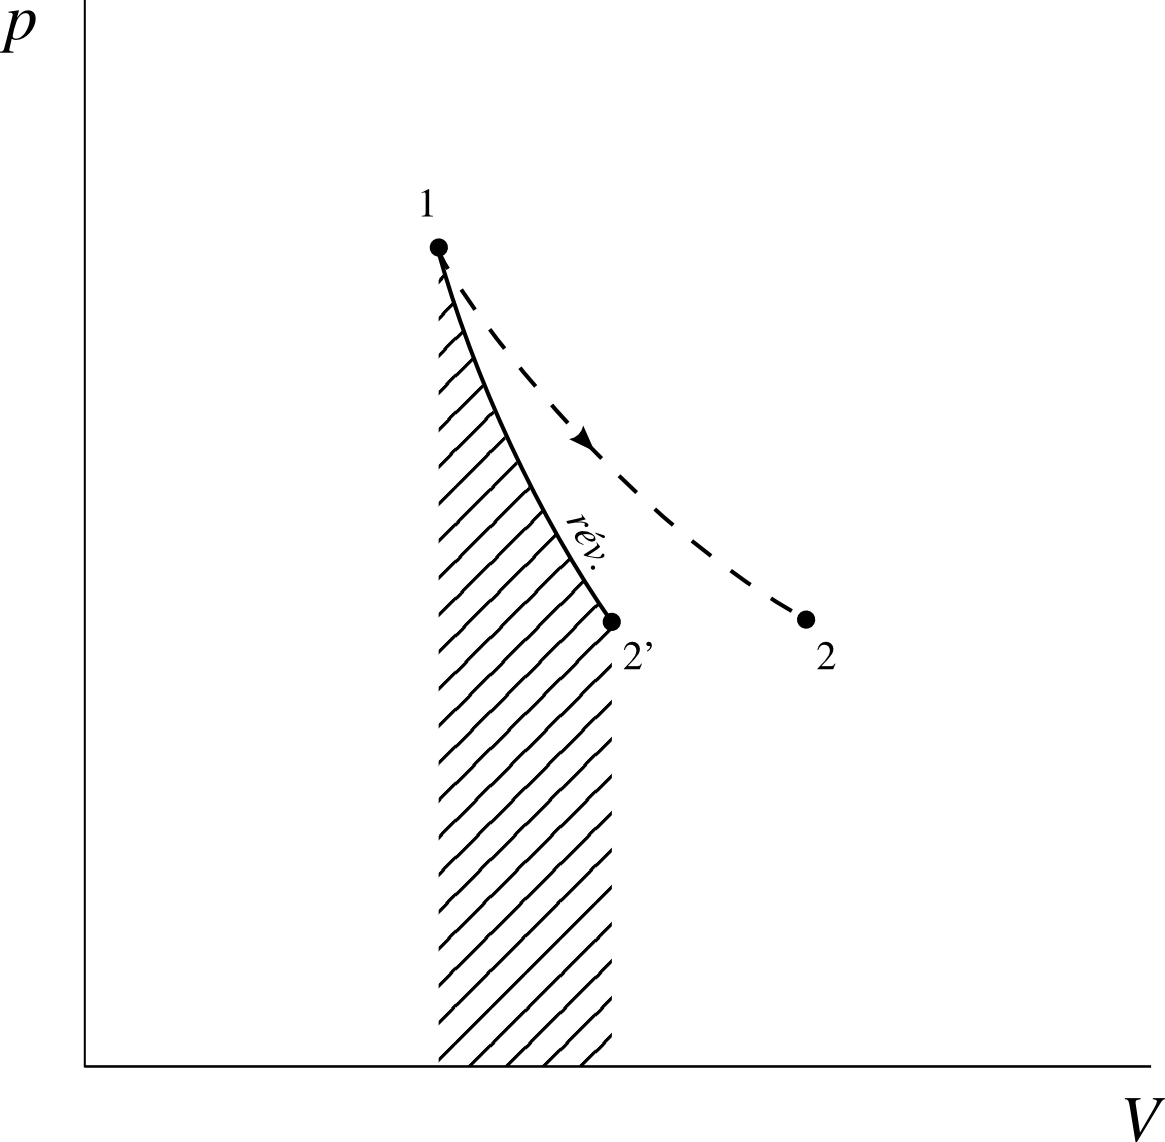
\includegraphics[width=9.5cm]{images/pv_reversible_irreversible.png}
			\end{center}
			\caption{Évolution du volume lors de détentes adiabatiques.
		L’augmentation du volume ne correspond à l’intégrale $\int (\diff W / p)_{\text{rév.}}$ que dans le cas d’un parcours réversible ($1 \to 2'$) , mais pas pour un parcours irréversible ($1 \to 2$).}
			\label{fig_pv_reversible_irreversible}
		\end{figure}

		\begin{figure}
			\begin{center}
				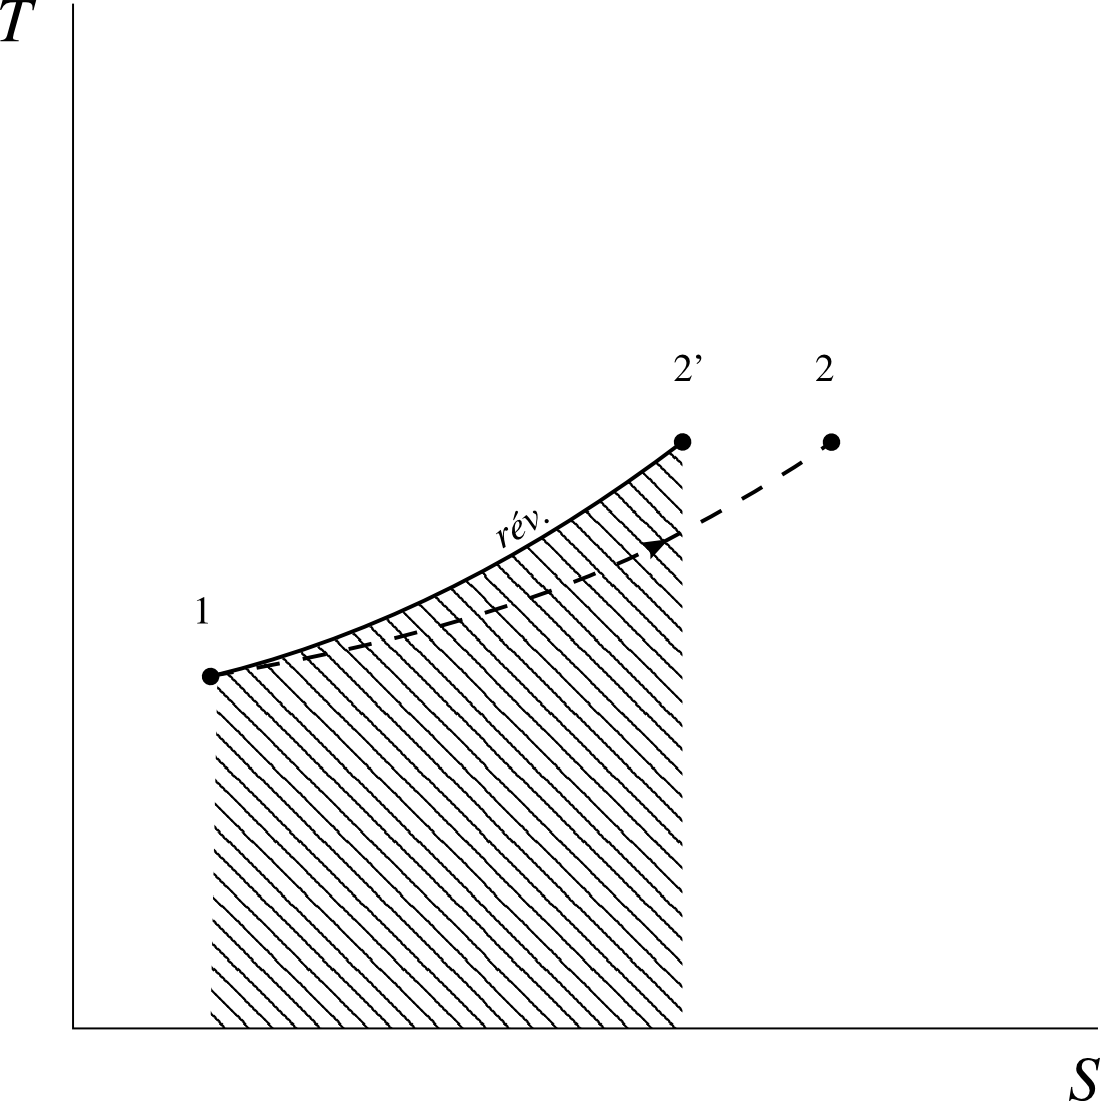
\includegraphics[width=9.5cm]{images/ts_reversible_irreversible.png}
			\end{center}
			\caption{Diagramme température-entropie. Lors d’une transformation réversible, l’aire sous la courbe d’un diagramme $T-S$ représente la chaleur transmise~$Q_{1 \to 2'}$ ; mais pas lorsqu’elle est irréversible.}
			\label{fig_ts_reversible_irreversible}
		\end{figure}

		Pour appréhender l’entropie, que l’on ne peut ni visualiser, ni mesurer directement, cette analogie avec le volume pourra peut-être aider l’étudiant/e.


 
	
	\subsection{Les diagrammes Température-entropie}
	
		Il est important pour nous de tracer les évolutions des fluides dans les machines sur un diagramme température-entropie. Cela nous permet de visualiser les transformations en jeu, exactement comme avec un diagramme pression-volume. À quoi ressemblent alors les principales évolutions sur un diagramme $T-s$ ?

		Lorsque le fluide reçoit ou fournit du travail de façon adiabatique réversible, alors $\Delta s = \int \frac{\diff q}{T} = 0$ puisque l’évolution est réversible et que $\diff q = 0$. Une transformation adiabatique réversible se fait donc à entropie constante --\ elle est iso-entropique, ce que nous appelons \vocab{isentropique}. Nous la représenterons ainsi par un trajet vertical sur les diagrammes température-entropie (\cref{fig_ts_basics}).

		\begin{figure}
			\begin{center}
				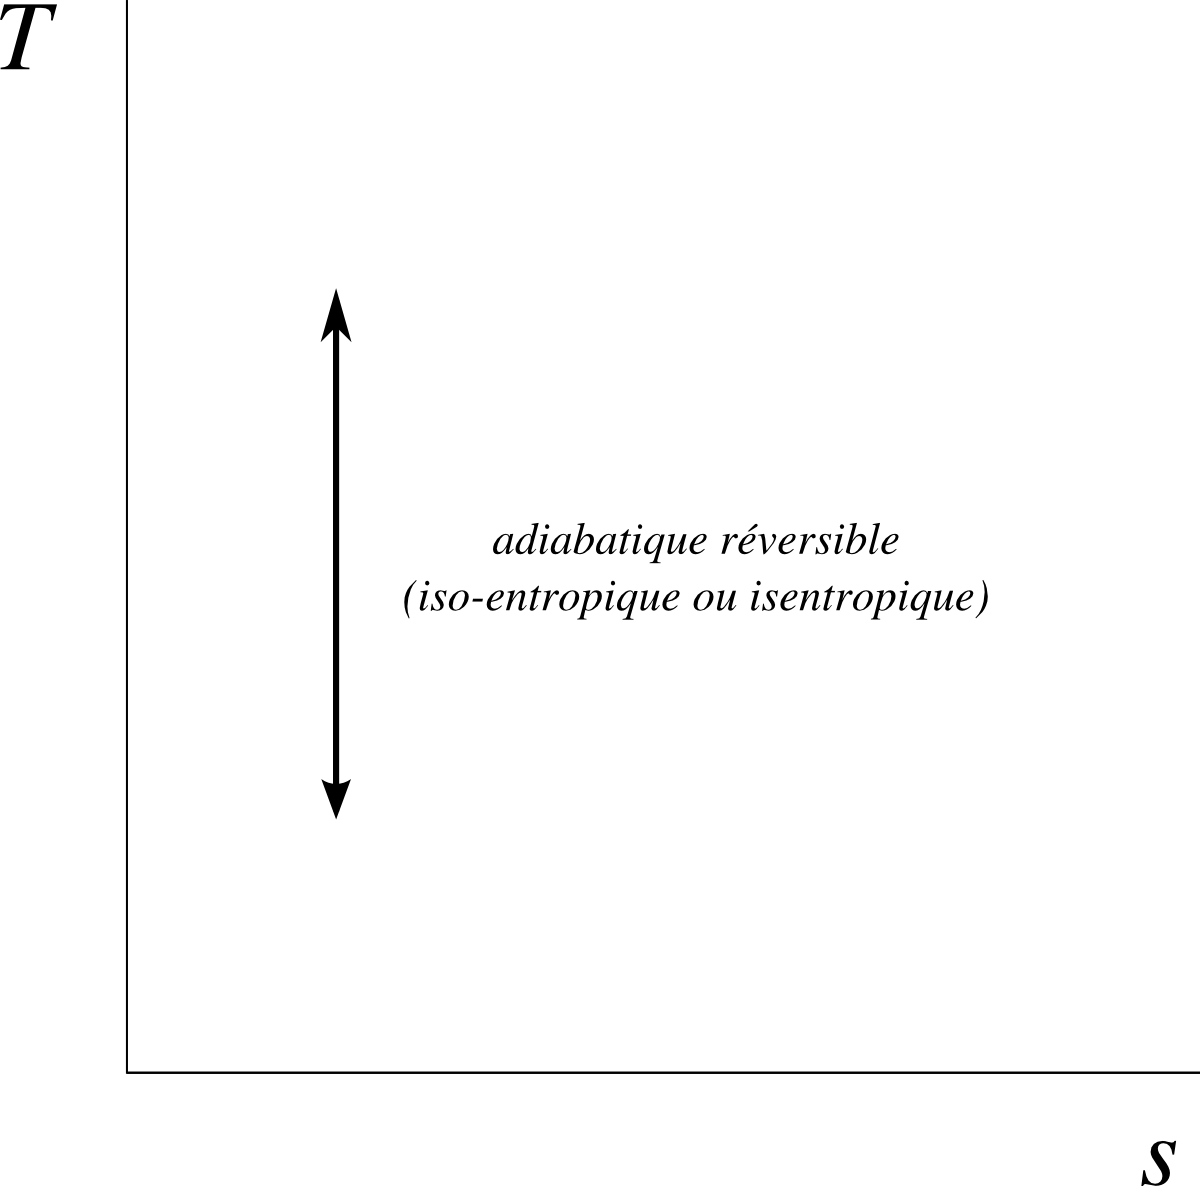
\includegraphics[width=0.45\textwidth]{images/ts_basics_1.png}
				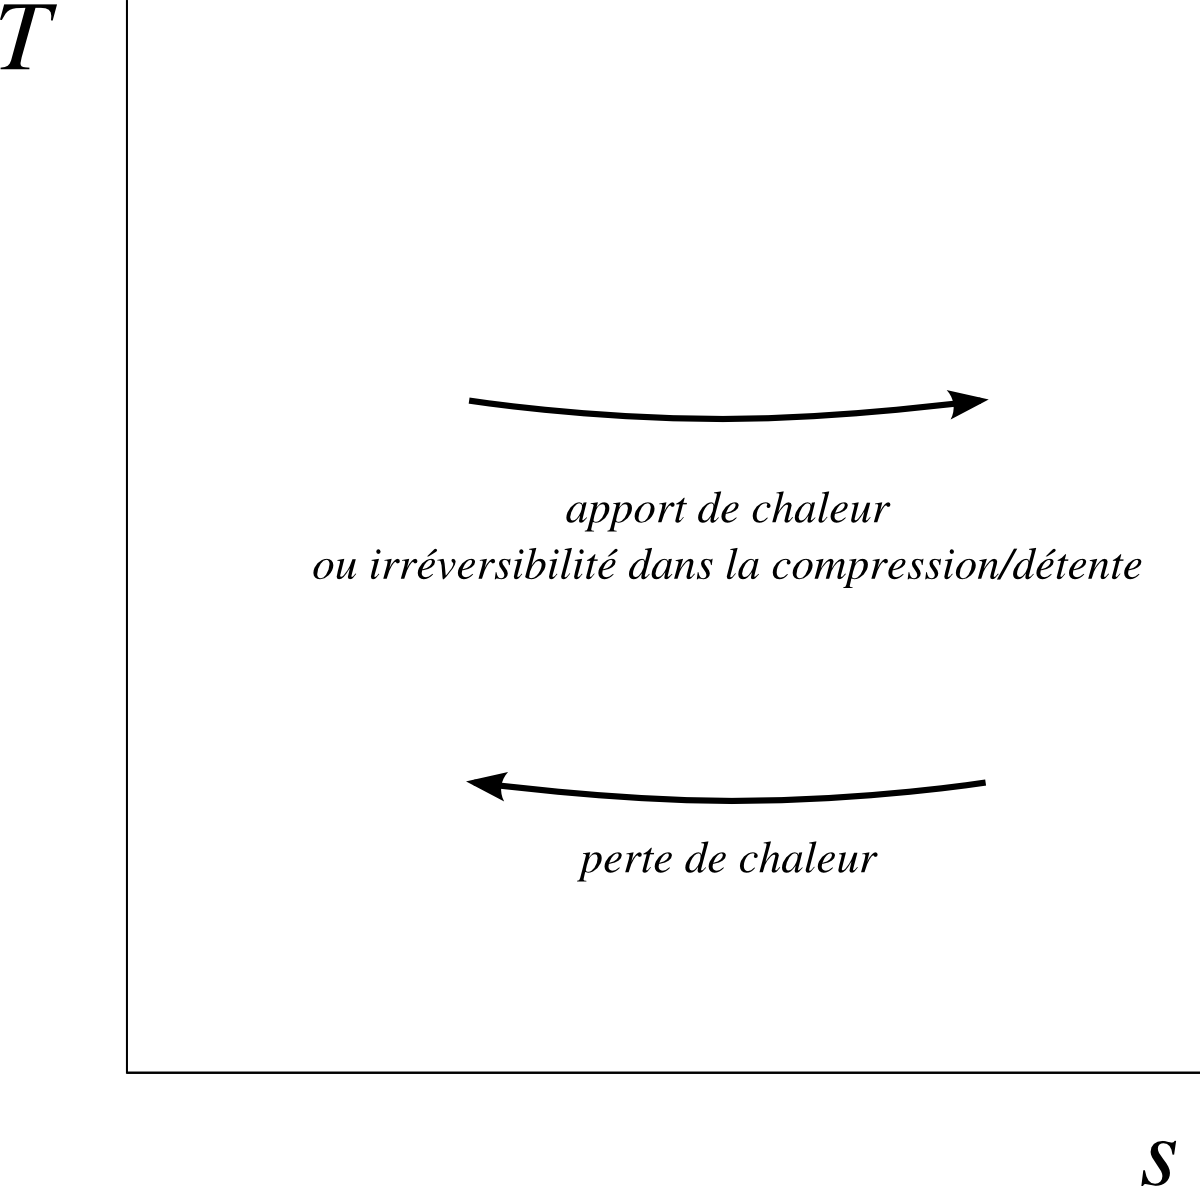
\includegraphics[width=0.45\textwidth]{images/ts_basics_2.png}
			\end{center}
			\caption{Évolutions élémentaires sur les diagrammes température-entropie.}
			\label{fig_ts_basics}
		\end{figure}

		Les transferts de chaleur, quant à eux, provoquent une variation de l’entropie du système (positive lorsque la chaleur est reçue, et négative lorsqu’elle est perdue). Sur les diagrammes $T-s$, nous nous déplacerons de gauche à droite lors des réceptions de chaleur ou bien lorsqu’il y a irréversibilité dans une compression ou une détente.

		Lorsque le système perd de la chaleur, son entropie décroît et nous nous déplacerons de droite à gauche sur les diagrammes $T-s$ (\cref{fig_ts_basics}).

		\clearfloats
		Notons aussi que, tout comme pour le volume, lorsqu’un fluide parcourt un cycle complet, il peut perdre son entropie à une température plus faible qu’il ne l’avait gagnée. La chaleur nette brassée est alors négative : le fluide a \emph{absorbé} de la chaleur\footnote{Cette chaleur aura été transformée en travail. En suivant le circuit inverse, le fluide produira une chaleur nette : c’est le principe du réfrigérateur (\S\ref{ch_principe_fonctionnement_réfrigérateur})}.


		Lorsque les évolutions sont réversibles, cette chaleur nette est représentée par l’aire enclose par le trajet sur un diagramme température-entropie (\cref{fig_ts_cycle}).

		\begin{figure}
			\begin{center}
				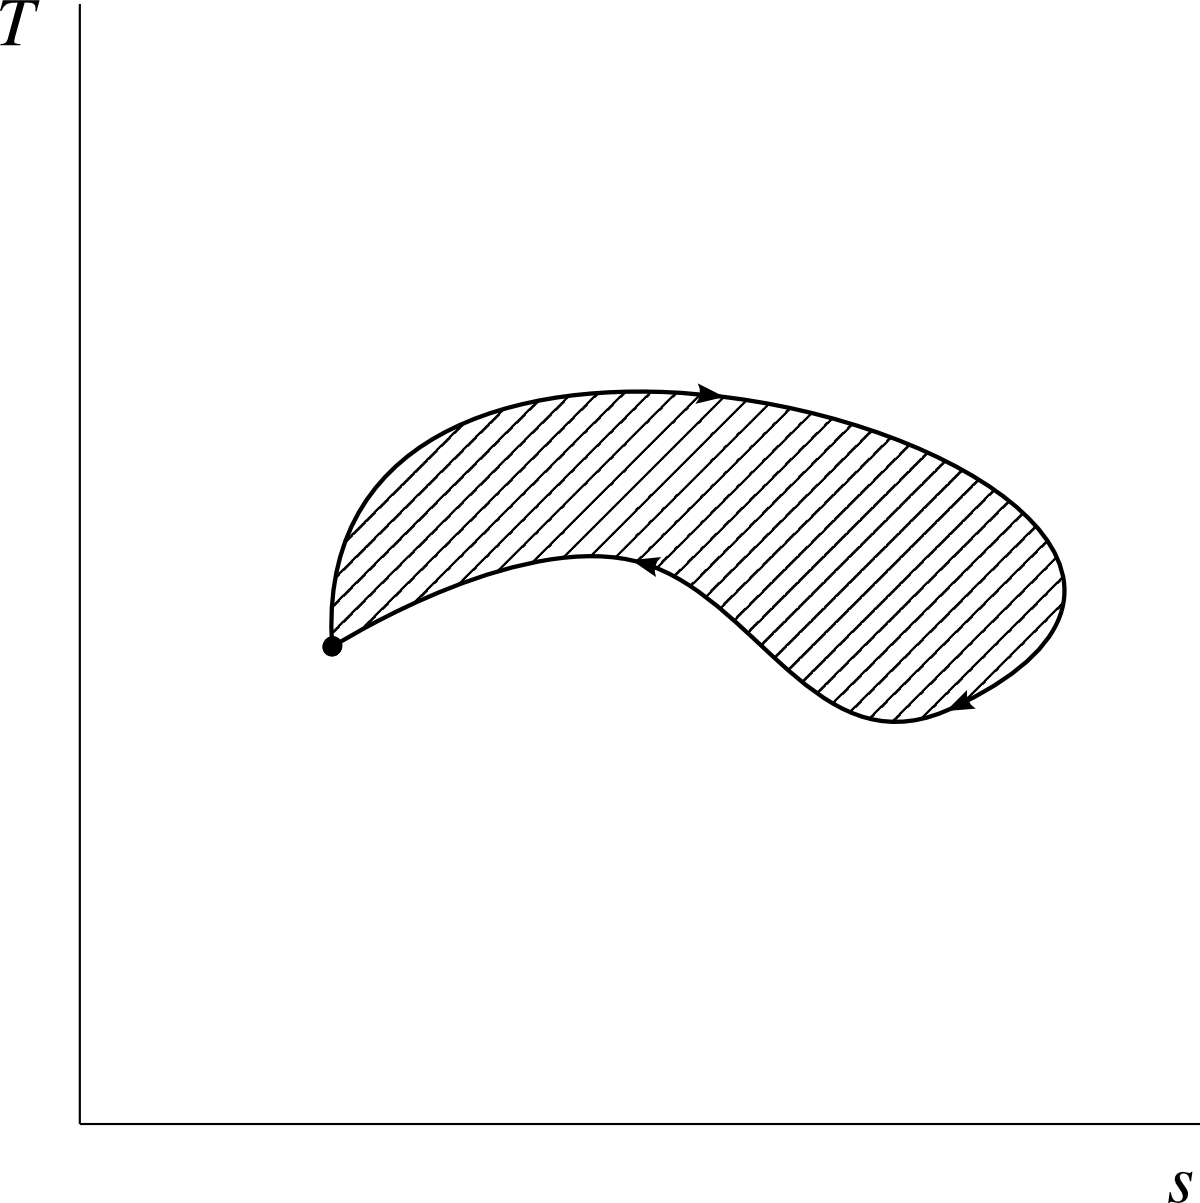
\includegraphics[width=9.5cm]{images/ts_cycle.png}
			\end{center}
			\caption{Cycle thermodynamique au cours duquel de la chaleur a été absorbée. Lorsque le trajet est effectué dans le sens inverse, de la chaleur est rejetée (transformée à partir de travail) par le fluide.}
			\label{fig_ts_cycle}
		\end{figure}

		\clearfloats
		Le cycle de Carnot, constitué de deux phases isothermes ($T = cst$) séparées par deux phases isentropiques ($s = cst$), gagne beaucoup à être représenté sur un diagramme température-entropie (\cref{fig_ts_carnot}).

		\begin{figure}
			\begin{center}
				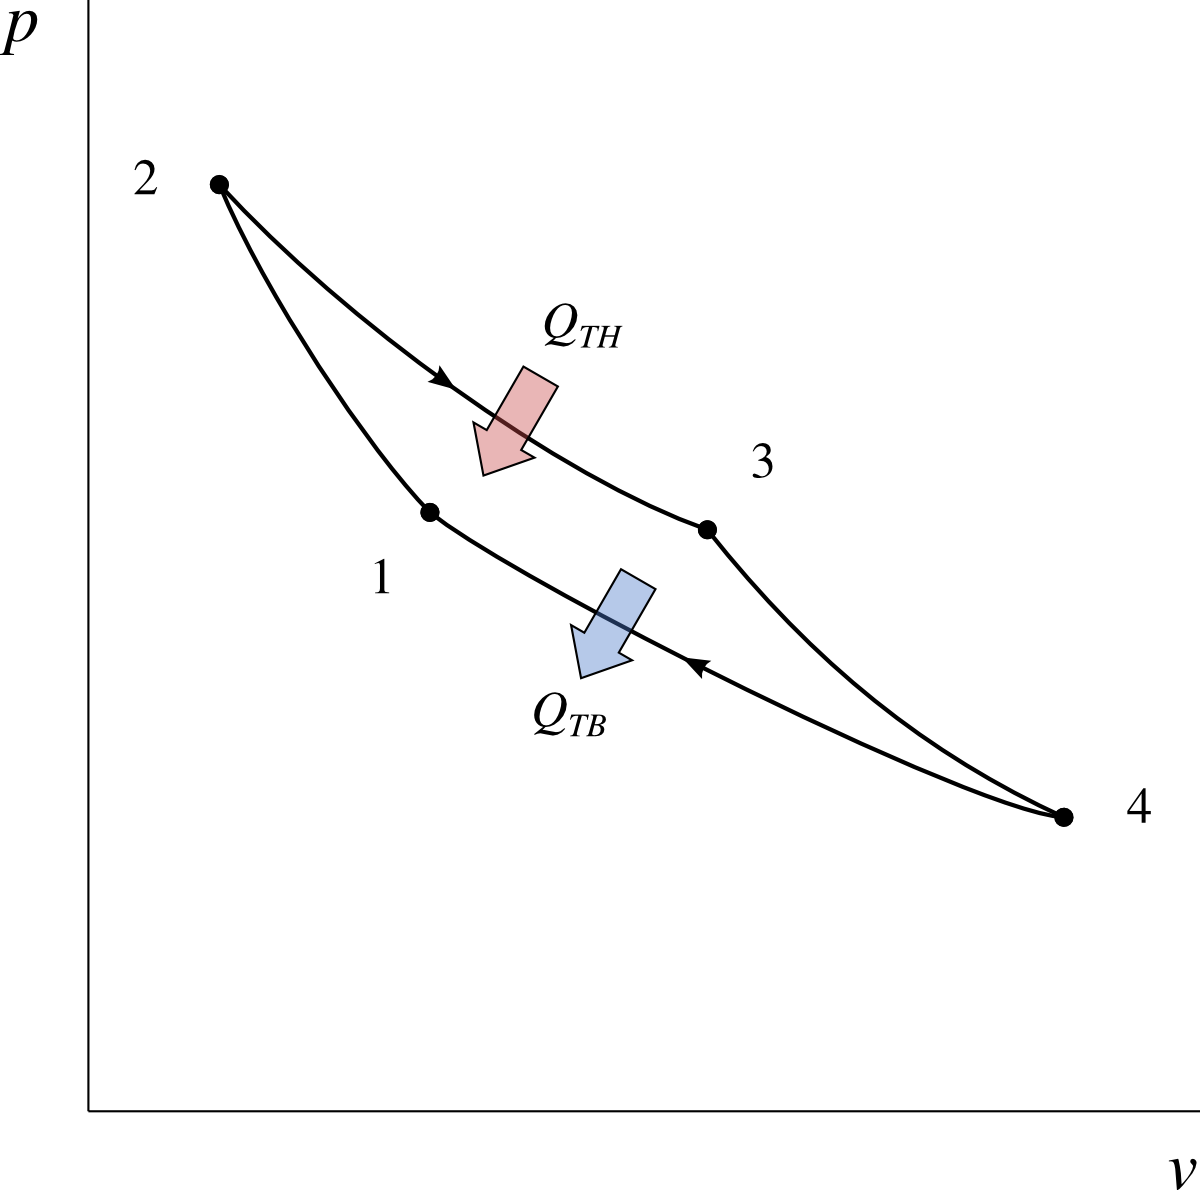
\includegraphics[width=0.49\textwidth]{images/pv_carnot_gp.png}
				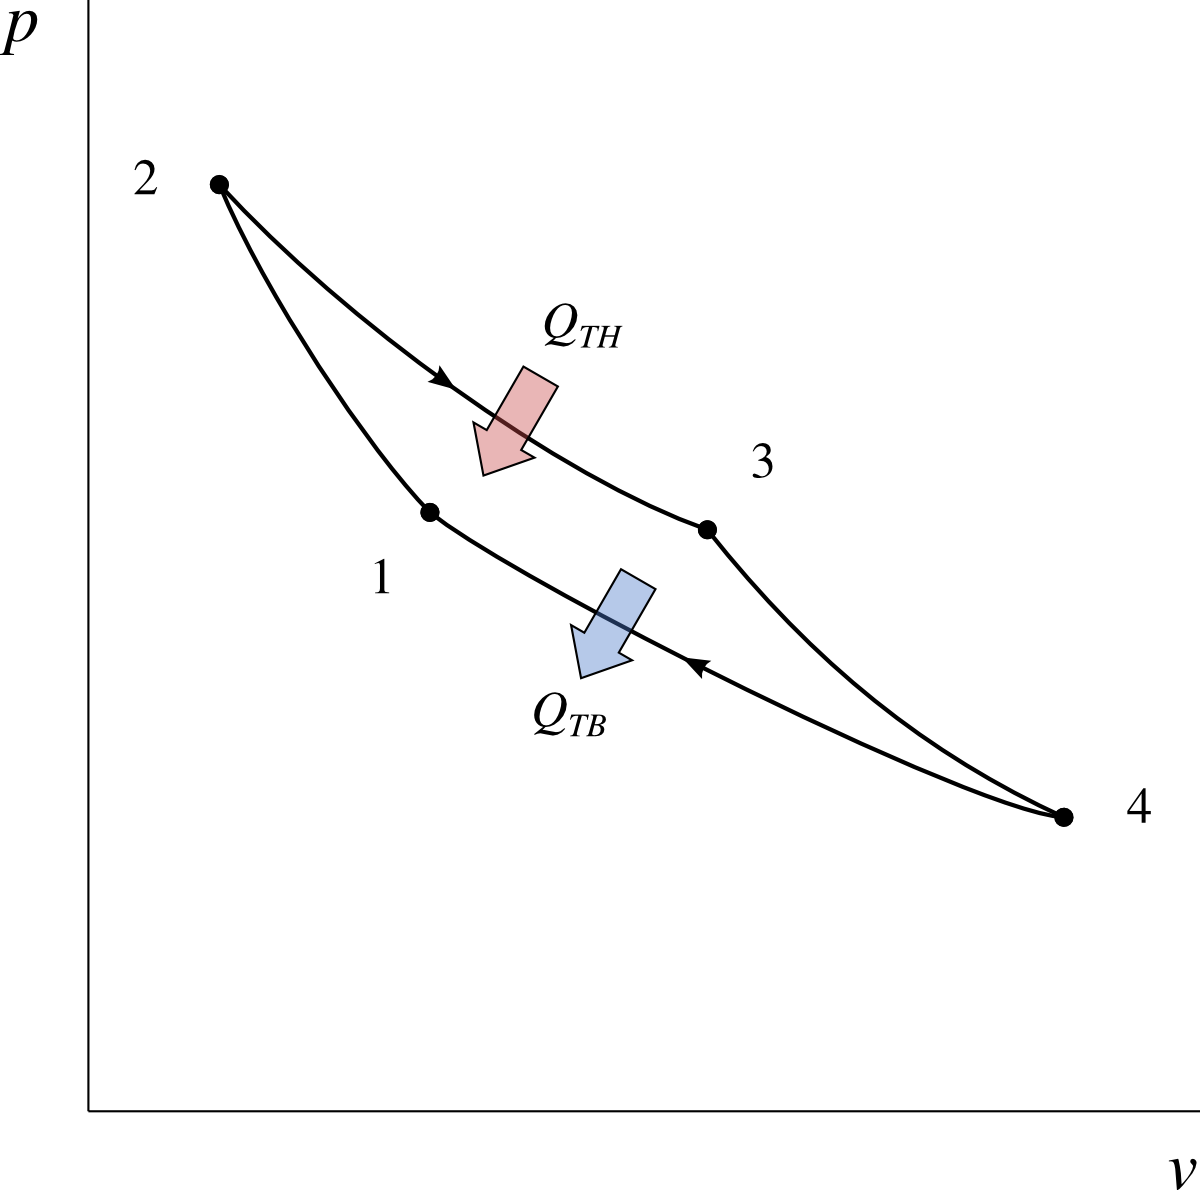
\includegraphics[width=0.49\textwidth]{images/pv_carnot_lv.png}
				\vspace{1cm}
				
				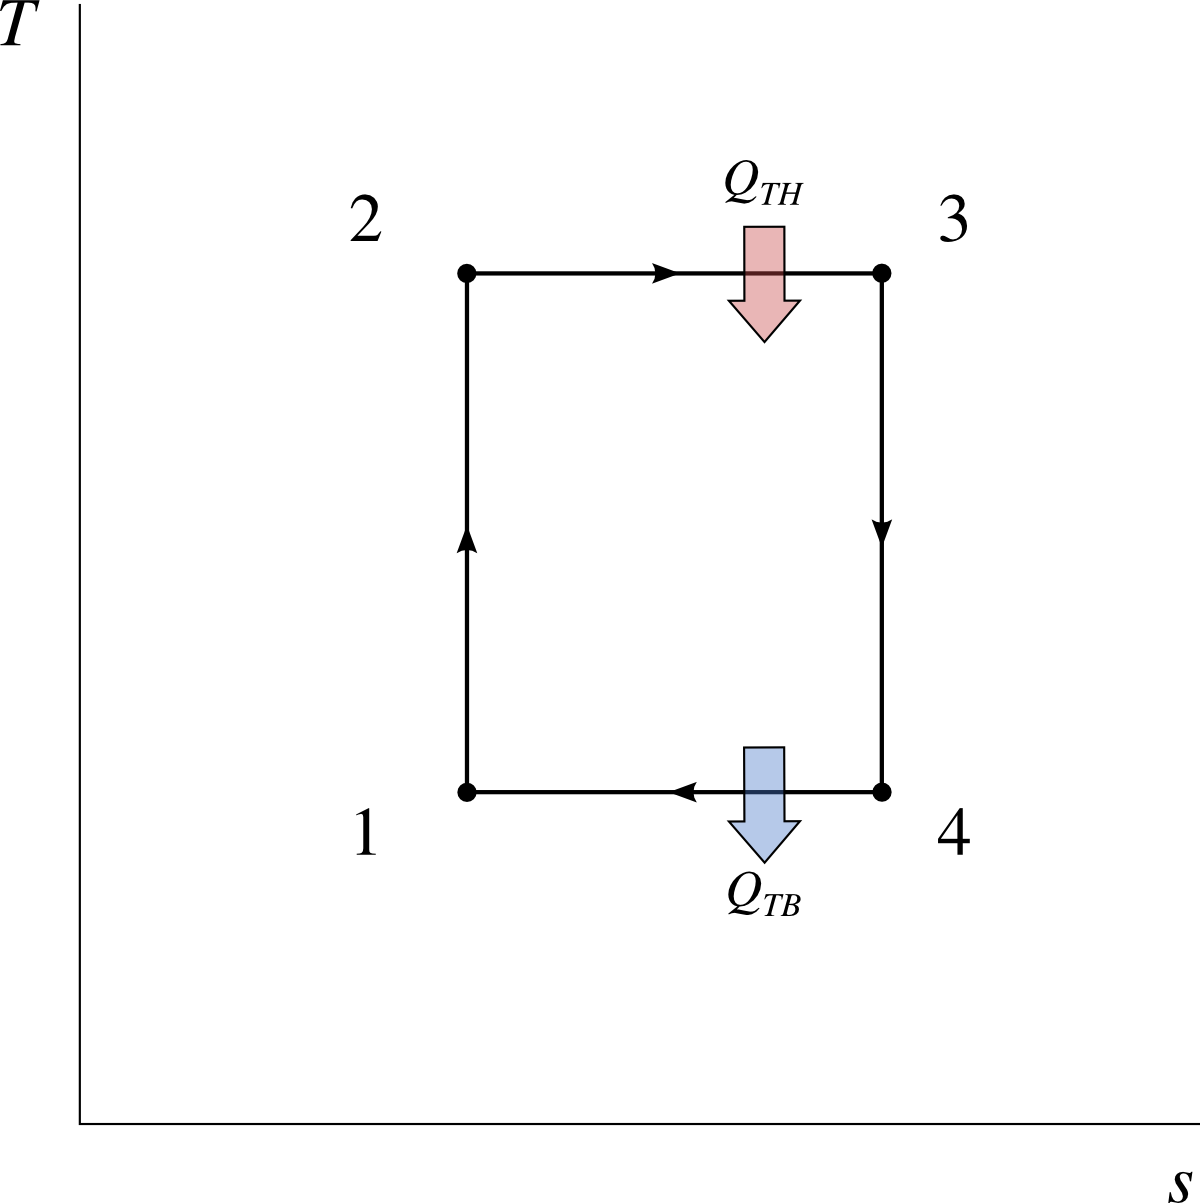
\includegraphics[width=8cm]{images/ts_carnot.png}
			\end{center}
			\caption{Cycle moteur de Carnot, sur un diagramme $p-v$ pour un gaz parfait (gauche), sur un diagramme $p-v$ pour un liquide-vapeur (droite), et sur un diagramme $T-s$ (bas). Quel que soit le fluide utilisé, le diagramme température-entropie reste le même.}
			\label{fig_ts_carnot}
		\end{figure}

	
	\subsection{Variations d’entropie d’un gaz parfait}
	\label{ch_delta_s_gaz_parfaits}
	
		Pour n’importe quelle évolution d’une quantité fixe de fluide, nous avons (\ref{eq_premier_principe_sf_min}) :
		
			\begin{equation*}
				q_{1\to2} + w_{1\to2} = \Delta u
			\end{equation*}
		
		Lorsque cette évolution est réversible, nous avons $q_{1\to2} = -\int_1^2 T \diff s$ (\ref{eq_q_tds_min}) et $w_{1\to2} = -\int_1^2 p \diff v$ (\ref{eq_travail_pdv}), et nous pouvons donc écrire :
			
			\begin{IEEEeqnarray}{rCl}
				\int_1^2 T \diff s - \int_1^2 p \diff v 	& = & \Delta u \nonumber\\
				T \diff s - p \diff v 							& = & \diff u \nonumber\\
				\diff s 												& = & \frac{\diff u}{T} + \frac{p}{T} \diff v \label{eq_delta_s_u_p_v_t}
			\end{IEEEeqnarray}
			
			\begin{equationterms}
				\item pour toute évolution réversible\footnote{Cette \cref{eq_delta_s_u_p_v_t} est même vraie pour toute évolution, mais cette généralisation est plus simple à aborder après les équations~\ref{eq_delta_s_gp_v} et~\ref{eq_delta_s_gp_p}.}\nolinebreak.
			\end{equationterms}
			
		Or, si nous utilisons un gaz parfait, nous avons $u = c_v T$ (\ref{eq_principe_de_joule})	et $\frac{p}{T} = \frac{R}{v}$ (\ref{eq_pv=RT}), ainsi :
				
			\begin{IEEEeqnarray}{rCl}
				\diff s 	& = & \frac{c_v \diff T}{T} + \frac{R}{v} \diff v \\
							& = & c_v\frac{\diff T}{T} + R \frac{\diff v}{v} \nonumber\\
				\Delta s	= s_2 - s_1 & = & c_v \ln \frac{T_2}{T_1} + R \ln \frac{v_2}{v_1} \label{eq_delta_s_gp_v}\\
				\Delta s	= s_2 - s_1 & = & c_p \ln \frac{T_2}{T_1} - R \ln \frac{p_2}{p_1} \label{eq_delta_s_gp_p}
			\end{IEEEeqnarray}
			
			\begin{equationterms}
				\item pour un gaz parfait,
				\item pour toute évolution de 1 à 2, réversible ou non.
			\end{equationterms}

		Cette équation est intéressante parce qu’elle nous indique que la variation d’entropie $\Delta s$ pendant une évolution de $1$ à $2$ ne dépend que des états finaux. Même si nous avons commencé cette démonstration avec une évolution réversible nous obtenons une expression~\ref{eq_delta_s_gp_v} dans laquelle le chemin utilisé n’apparaît pas. 
		
		Il est donc possible de calculer la variation d’entropie d’un gaz parfait si l’on connaît ses autres propriétés. Contrairement à l’énergie interne $u$ qui ne dépend que de la température, l’entropie $s$ dépend aussi de la pression du gaz.

		Dans le cas où la pression ou le volume spécifique sont maintenus constants, il est facile de montrer que ces équations~\ref{eq_delta_s_gp_v} et~\ref{eq_delta_s_gp_p} deviennent respectivement :
			
			\begin{IEEEeqnarray}{rCl}
				\Delta s_{v_\text{cst.}} 		& = & c_v \ln \frac{T_2}{T_1} 	\label{eq_delta_s_gp_vcst} \\
				\Delta s_{p_\text{cste}} 	& = & c_p \ln \frac{T_2}{T_1} 	\label{eq_delta_s_gp_pcste}
			\end{IEEEeqnarray}
	
			\begin{equationterms}
				\item pour un gaz parfait,
				\item pour toute évolution à volume constant ou respectivement à pression constante.
			\end{equationterms}

		Ces deux équations~\ref{eq_delta_s_gp_vcst} et~\ref{eq_delta_s_gp_pcste} nous permettent de tracer des courbes isochores (à volume constant) et isobares (à pression constante) pour un gaz parfait sur un diagramme $T-s$, comme montré en \cref{fig_ts_gp_isobares_isochores}.

		\begin{figure}
			\begin{center}
				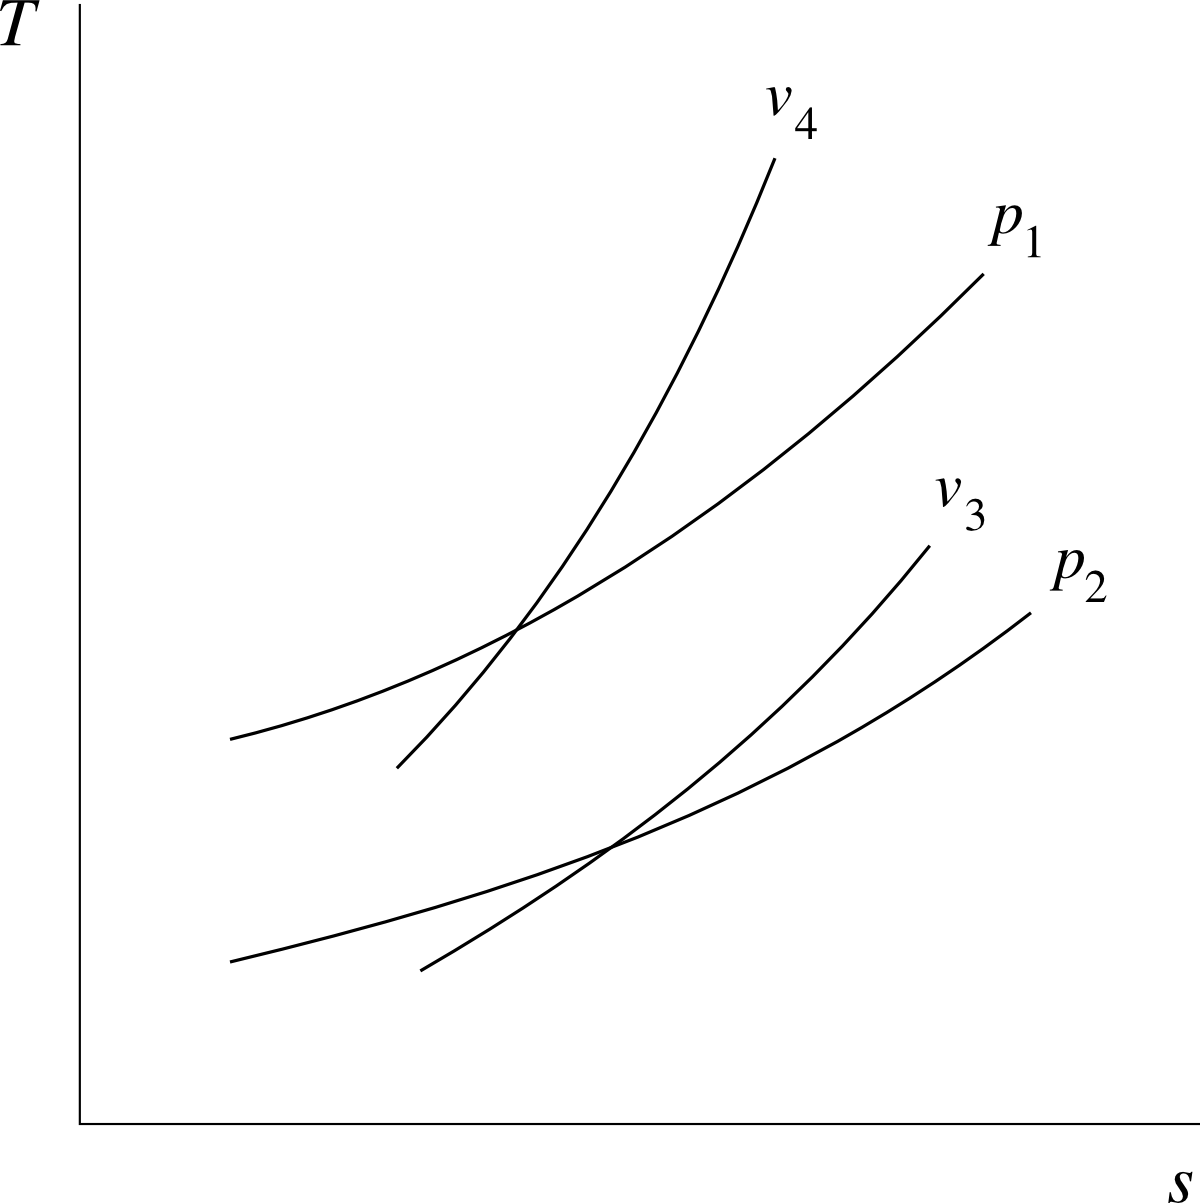
\includegraphics[width=9.5cm]{images/ts_gp_isobares_isochores.png}
			\end{center}
			\caption{Courbes isobares et isochores sur un diagramme $T-s$, pour un gaz parfait.
		Ici $p_1>p_2$ et $v_3>v_4$.}
			\label{fig_ts_gp_isobares_isochores}
		\end{figure}

		\clearfloats
		\begin{anexample}
			Quelle est la variation d’entropie spécifique d’une masse de~\SI{2}{\kilogram} d’air, lorsqu’elle est chauffée à pression constante de~\SI{2}{\bar}, depuis \SI{10}{\degreeCelsius} jusqu’à~\SI{100}{\degreeCelsius} ?
			
				\begin{answer}
					L’évolution peut être dessinée de façon approximative sur un diagramme $T-s$ :\\
						\begin{center}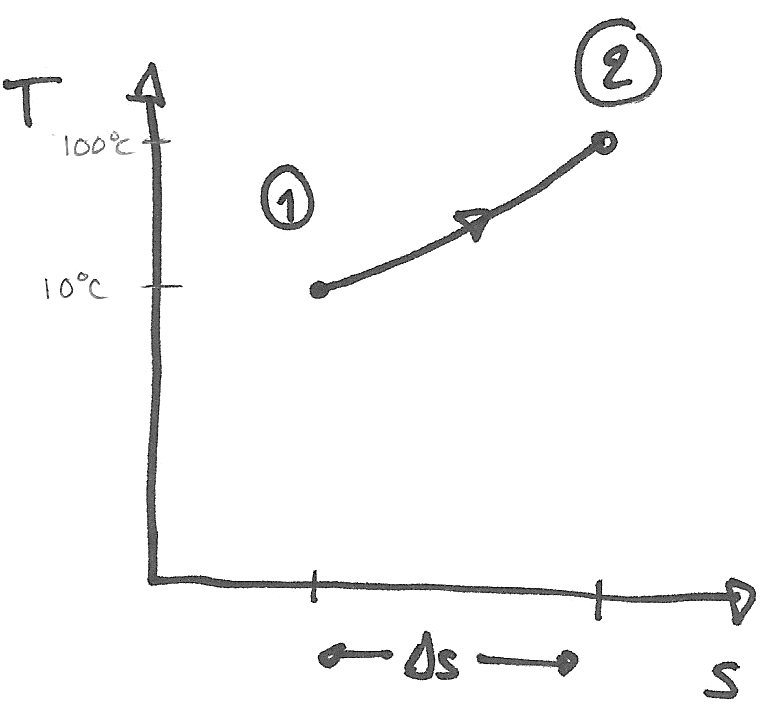
\includegraphics[width=6cm]{images/ts_example_1.png}\end{center}
					Pour calculer $\Delta S$ nous partons de l’\cref{eq_delta_s_gp_p}, $\Delta s = c_p \ln \frac{T_2}{T_1} - R \ln \frac{p_2}{p_1}$ et ici $p_2=p_1$. Nous avons donc $\Delta s = c_p \ln \frac{T_2}{T_1} = \num{1005} \ln \frac{100+273,15}{10+273,15} =  \SI{+277,4}{\joule\per\kelvin\per\kilogram}$. \\L’entropie varie donc de $\Delta S = m \Delta s = 2 \times 277,4 = \SI{+554,8}{\joule\per\kelvin}$. 
				
				\begin{remark}Nous écrivons bien que «~l’entropie de l’air augmente~» et non pas qu’«~on lui donne de l’entropie~» (\S\ref{ch_entropie_propriete}).\end{remark}\end{answer}
		\end{anexample}


		\begin{anexample}
			De combien varie l’entropie d’une masse d’air de~\SI{0,5}{\kilogram} refroidie lentement à température constante depuis \SI{1}{\bar} et~\SI{50}{\degreeCelsius} jusqu’à~\SI{5}{\bar} ? Combien faut-il lui prendre de chaleur pour cela ?
			
				\begin{answer}
					L’évolution peut être dessinée de façon approximative sur un diagramme $T-s$ :\\
						\begin{center}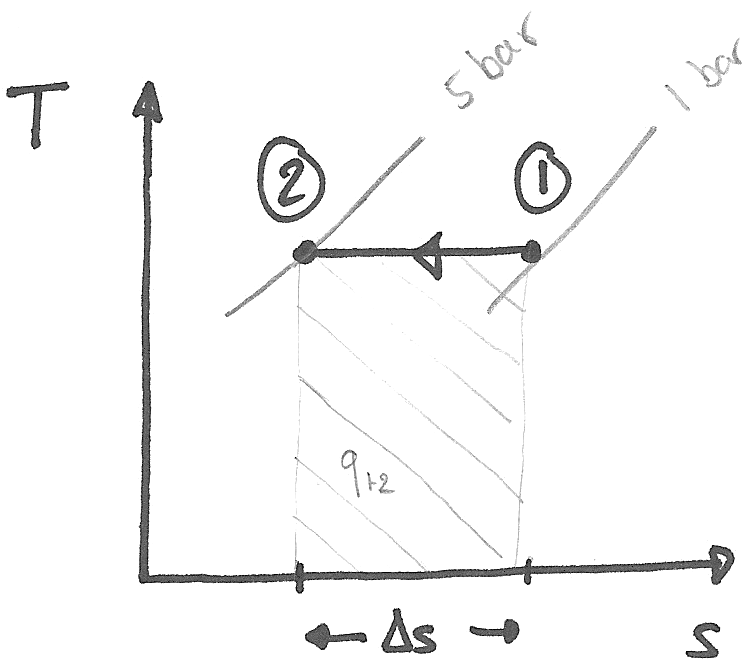
\includegraphics[width=6cm]{images/ts_example_2.png}\end{center}
					Pour quantifier $\Delta S$ nous partons de l’\cref{eq_delta_s_gp_p}, $\Delta s = c_p \ln \frac{T_2}{T_1} - R \ln \frac{p_2}{p_1}$ et ici $T_2=T_1$. Nous avons donc $\Delta s = -R \ln \frac{p_2}{p_1} = \num{287} \ln \frac{5}{1} =  \SI{-461,9}{\joule\per\kelvin\per\kilogram}$. \\L’entropie varie donc de $\Delta S = m \Delta s = \num{0,5} \times \num{-461,9} = \SI{-231}{\joule\per\kelvin}$. 
					
					Comme l’évolution est réversible, la chaleur prélevée s’obtient avec l’\cref{eq_q_tds_maj} : $Q_{1\to2} = \int_1^2 T \diff S = T_\text{cste} \int_1^2 \diff S = T_\text{cste} \Delta S = (50+273,15) \times \num{-231} = \SI{-74,6}{\kilo\joule}$. 
				
				\begin{remark}Nous savions déjà quantifier $Q_{1\to2}$ sans utiliser l’entropie, à l’aide des équations \ref{eq_gp_travail_isotherme_sf} et \ref{eq_gp_chaleur_isotherme_sf}.\end{remark}\end{answer}
		\end{anexample}

		\begin{anexample}
			De combien varie la température d’une masse d’air détendue de façon adiabatique réversible depuis \SI{30}{\bar} et~\SI{600}{\kelvin} jusqu’à~\SI{1}{\bar} ?
			
				\begin{answer}
					L’évolution peut être dessinée de façon approximative sur un diagramme $T-s$ :\\
						\begin{center}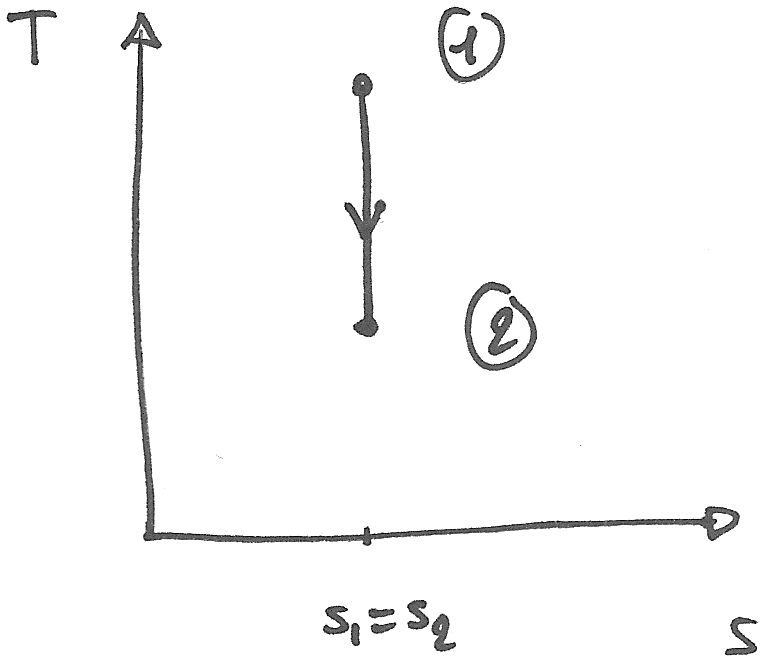
\includegraphics[width=6cm]{images/ts_example_3.png}\end{center}
					Pour quantifier $\Delta S$ nous partons encore de l’\cref{eq_delta_s_gp_p} : $\Delta s = c_p \ln \frac{T_2}{T_1} - R \ln \frac{p_2}{p_1}$ et ici $\Delta s = 0$ :\vspace{-1cm}
					
						\begin{IEEEeqnarray*}{rCl}
							0 										& = & c_p \ln \frac{T_2}{T_1} - R \ln \frac{p_2}{p_1} \\
							\ln \frac{T_2}{T_1}				& = & \frac{R}{c_p} \ln \frac{p_2}{p_1} \\
							\left(\frac{T_2}{T_1}\right)	& = & \left(\frac{p_2}{p_1}\right)^{\frac{R}{c_p}} = \left(\frac{p_2}{p_1}\right)^{\frac{\gamma-1}{\gamma}}
						\end{IEEEeqnarray*}
				
					Nous reconnaissons ainsi l’\cref{eq_isentropique_horrible2} que nous savons déjà appliquer : $T_2 = 600 \times \frac{1}{30}^{\frac{0,4}{1,4}} =  \SI{227}{\kelvin} $, soit environ \SI{-46}{\degreeCelsius}.
				
				\begin{remark}L’utilisation du raisonnement «~adiabatique réversible = isentropique~» ne nous a, en vérité, rien apporté que nous ne savions déjà ici, car le modèle du gaz parfait est déjà extrêmement simple et puissant. Ce ne sera pas le cas avec les liquides/vapeurs.\end{remark}\end{answer}
		\end{anexample}
	
	\subsection{Variations d’entropie d’un liquide/vapeur}
	
		Pour un liquide/vapeur, les variations ne peuvent pas être calculées car il n’existe pas de modèle mathématique simple pour modéliser la température. La courbe de saturation et le chemin d’une évolution à pression constante sont représentés en \cref{fig_ts_lv} ; cette figure~ressemble très fortement au diagramme température-volume que nous avions tracé en \cref{fig_t-v_eau}.
		Pour quantifier les valeurs de $s$, nous allons procéder exactement comme avec l’énergie interne $u$ au \courscinq : en les tabulant.

		\begin{figure}
			\begin{center}
				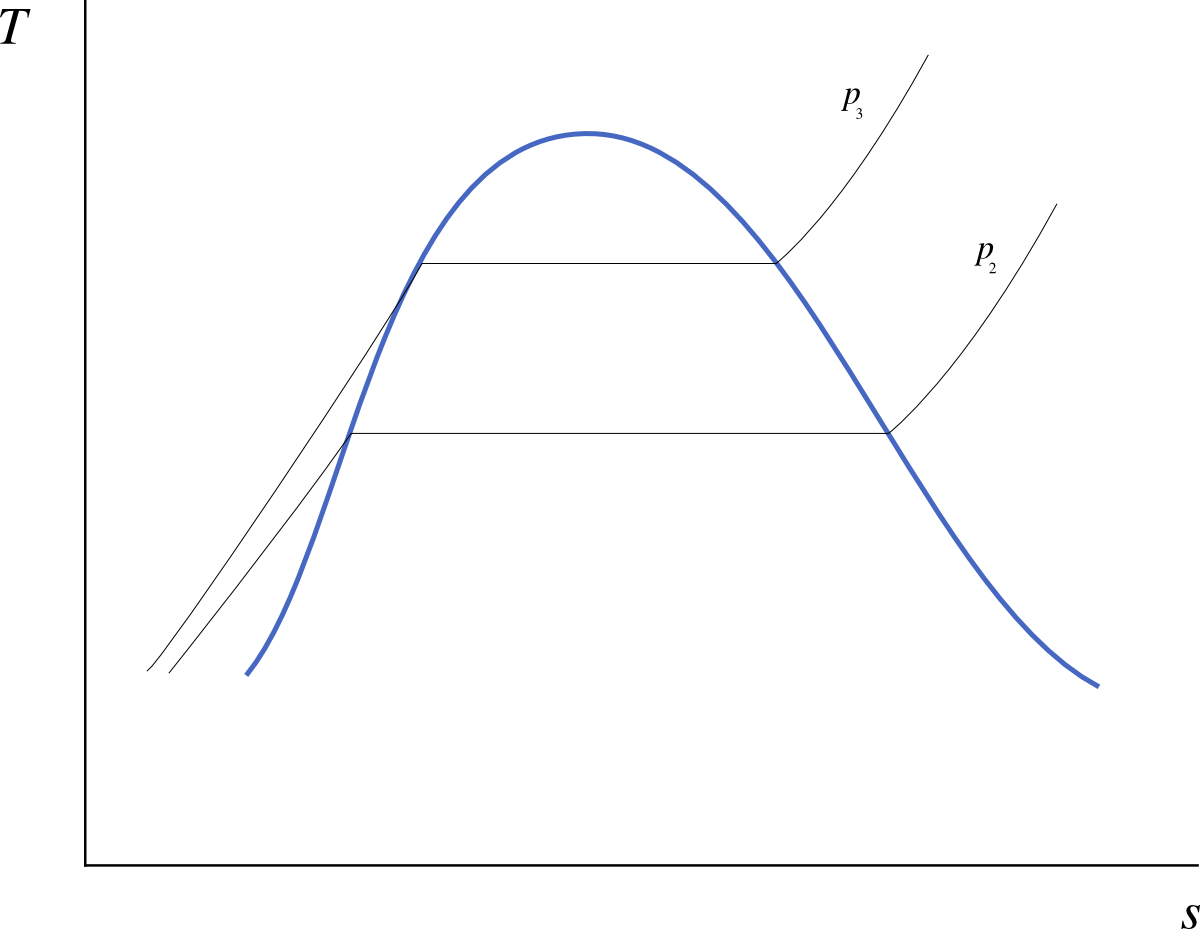
\includegraphics[width=9.5cm]{images/ts_lv.png}
			\end{center}
			\caption{Diagramme température-entropie d’un liquide/vapeur. Cette figure est très similaire à la \cref{fig_t-v_eau}.}
			\label{fig_ts_lv}
		\end{figure}
		
		En dehors des phases de mélange (c’est-à-dire lorsque l’eau est à l’état de liquide comprimé ou de vapeur sèche) l’entropie\footnote{En réalité, \emph{toutes} les valeurs tabulées de l’entropie sont relatives à un point de référence pour lequel la valeur de $s$ est arbitrairement posée à~\SI{0}{\joule\per\kelvin\per\kilogram} ; dans notre cas, c’est le point triple de l’eau. Cela n’a pas d’importance dans nos calculs puisque seules les variations de l’entropie nous intéressent.} peut simplement être lue en dernière colonne dans l’abaque~n°1, dont un extrait est répété en \cref{tab_abaque1extraitbis}.
		
		\begin{table}
		\begin{center}
		\begin{footnotesize}
		\begin{tabular}{
		|S[table-format = 4.0]|%				T
		S[table-format = 2.6]% 		v
		S[table-format = 4.1]%			u
		S[table-format = 4.1]%		h
		S[table-format = 2.4]|%	s
		}

 		\hline
		%\addlinespace[10pt]
		 &&&&\\
		\multicolumn{1}{|@{}c@{}|}{{\scriptsize °C}}	% Using SIunit screws the table up here for some reason
		&\multicolumn{1}{@{}c@{}}{{\small\si[per-mode = fraction]{\metre\cubed\per\kilogram}}}%
		&\multicolumn{1}{@{}c@{}}{{\small\si[per-mode = fraction]{\kilo\joule\per\kilogram}}}%
		&\multicolumn{1}{@{}c@{}}{{\small\si[per-mode = fraction]{\kilo\joule\per\kilogram}}}%
		&\multicolumn{1}{@{}c@{}|}{{\small\si[per-mode = fraction]{\kilo\joule\per\kilogram\per\kelvin}}}\\%

		%\addlinespace[10pt]
		 &&&&\\
		{$T$}	&$v$	&$u$	&$h$	&$s$\\
		\hline
 		
		&\multicolumn{4}{c|}{$p = \SI{1,6}{\mega\pascal}$}\\
		&\multicolumn{4}{c|}{($T_\text{sat} = \SI{201,37}{\degreeCelsius}$)}\\
		
		10		&0,001		&42		&43,6		&0,1509\\
		20		&0,001001	&83,8		&85,4		&0,2962\\
		50		&0,001011	&209,1	&210,7	&0,7031\\
		100	&0,001043	&418,6	&420,3	&1,306\\
		200	&0,001156	&850,4	&852,3	&2,3305\\	\cdashline{2-5}[.8pt/2pt]
		300	&0,15866	&2781,5	&3035,4	&6,8863\\
		500	&0,22029	&3120,1	&3472,6	&7,5409\\
		600	&0,24999	&3293,9	&3693,9	&7,81\\
		700	&0,2794	&3473,5	&3920,5	&8,0557\\
		800	&0,30865	&3659,5	&4153,3	&8,2834\\
		900	&0,3378	&3852,1	&4392,6	&8,4965\\
		1000	&0,36687	&4051,2	&4638,2	&8,6974\\
		1100	&0,39589	&4256,6	&4890		&8,8878\\
		1200	&0,42487	&4467,9	&5147,7	&9,0689\\
		1500	&0,51169	&5133,7	&5952,4	&9,5656\\
		2000	&0,65615	&6326,8	&7376,6	&10,272\\
		\hline

 		\end{tabular}\end{footnotesize}\end{center}
 		\caption{Extrait de l’abaque~n°1. L’entropie peut être lue en dernière colonne et ses valeurs interpolées comme les autres propriétés.}
 		\label{tab_abaque1extraitbis}
 		\end{table}

	
		À l’intérieur de la courbe de saturation les valeurs de $s$ s’interpolent entre celles de $s_L$ (liquide saturé) et $s_V$ (vapeur saturée) à l’aide de la notion de \emph{titre}, exactement comme avec l’\cref{eq_titre_energie_interne} :
		
		\begin{equation}
			s_x = s_L + x \ s_{LV}
			\label{eq_titre_entropie}
		\end{equation}
	
		\clearfloats
		\begin{anexample}
			Quelle est la variation de l’entropie de l’eau lorsqu’elle part d’un état à~\SI{240}{\degreeCelsius} et~\SI{6}{\bar}, pour arriver à~\SI{130}{\degreeCelsius} avec une énergie interne de~\SI{1000}{\kilo\joule\per\kilogram} ?% surch → mélange liq/v
			
				\begin{answer}
					Après un coup d’œil aux abaques, l’évolution peut être dessinée de façon approximative sur un diagramme $T-s$ :\\
						\begin{center}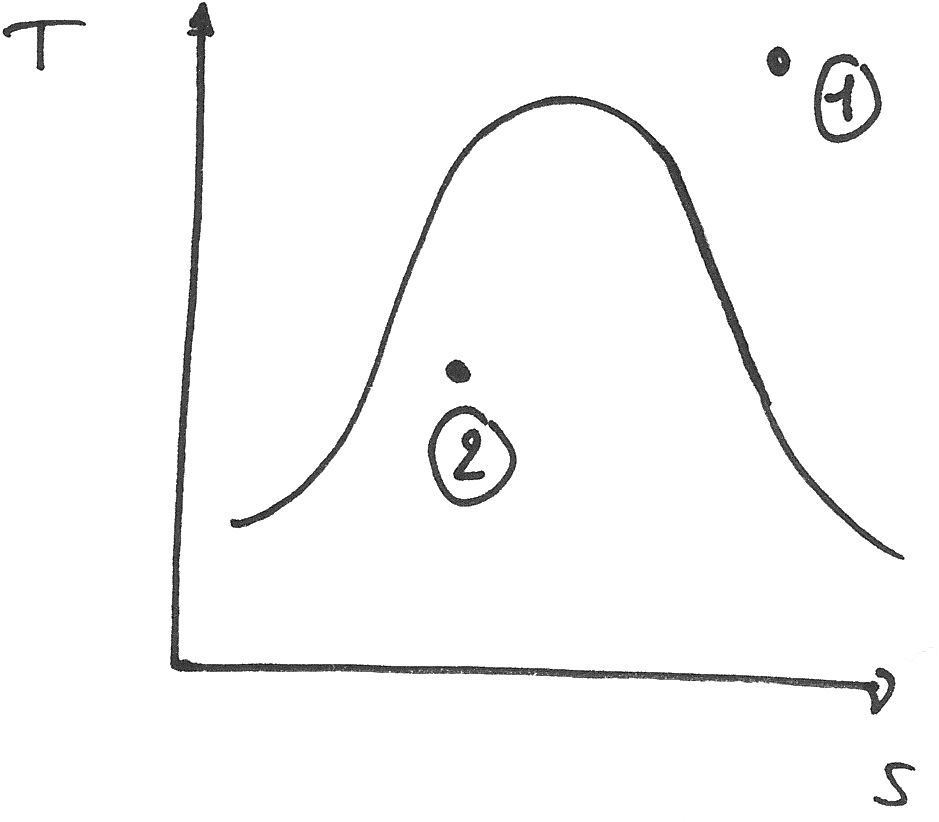
\includegraphics[width=6cm]{images/ts_example_4.png}\end{center}
					Nous lisons $s_1$ par interpolation dans l’abaque n°1 à~\SI{0,6}{\mega\pascal} entre \SI{200}{\degreeCelsius} et~\SI{300}{\degreeCelsius} : $s_1= \num{6,9683} + \frac{40}{100}\times(\num{7,374}-\num{6,9683}) = \SI{7,1306}{\kilo\joule\per\kelvin\per\kilogram} $.\\
					À l’arrivée, l’eau est en mélange liquide-vapeur (puisque $u_2<u_{V\SI{130}{\degreeCelsius}}$), nous lisons donc en abaque n°2 (\ref{eq_titre_energie_interne}) : $x_2 = \frac{u_2 - u_L}{u_{LV}} = \frac{\num{1000}-\num{546,1}}{\num{1993,5}}= \num{0,228} $ ; ainsi avec l’\cref{eq_titre_entropie} nous pouvons calculer l’entropie : $s_2= s_L + x_2 \ s_{LV} = \num{1,6346}+ \num{0,228}\times\num{5,3918} = \SI{2,8623}{\kilo\joule\per\kelvin\per\kilogram}$.\\
					Nous voyons que l’entropie a diminué : $\Delta s = s_2 - s_1 = \SI{-4,268}{\kilo\joule\per\kelvin\per\kilogram} $.
				
				\begin{remark}Nous ne savons pas quelle transformation a eu lieu. Moins elle a été réversible, et plus il aura fallu retirer de la chaleur à la vapeur pour l’amener de 1 à 2.\end{remark}\end{answer}
		\end{anexample}

		
		\begin{anexample}
			On réchauffe lentement \SI{2}{\kilogram} d’eau liquide saturée à~\SI{300}{\degreeCelsius}, en maintenant sa température constante, jusqu’à ce que le volume atteigne \SI{2}{\metre\cubed}. Combien faut-il apporter de chaleur pour cela ?
			
				\begin{answer}
					Après un coup d’œil aux abaques, l’évolution peut être dessinée de façon approximative sur un diagramme $T-s$ :\\
						\begin{center}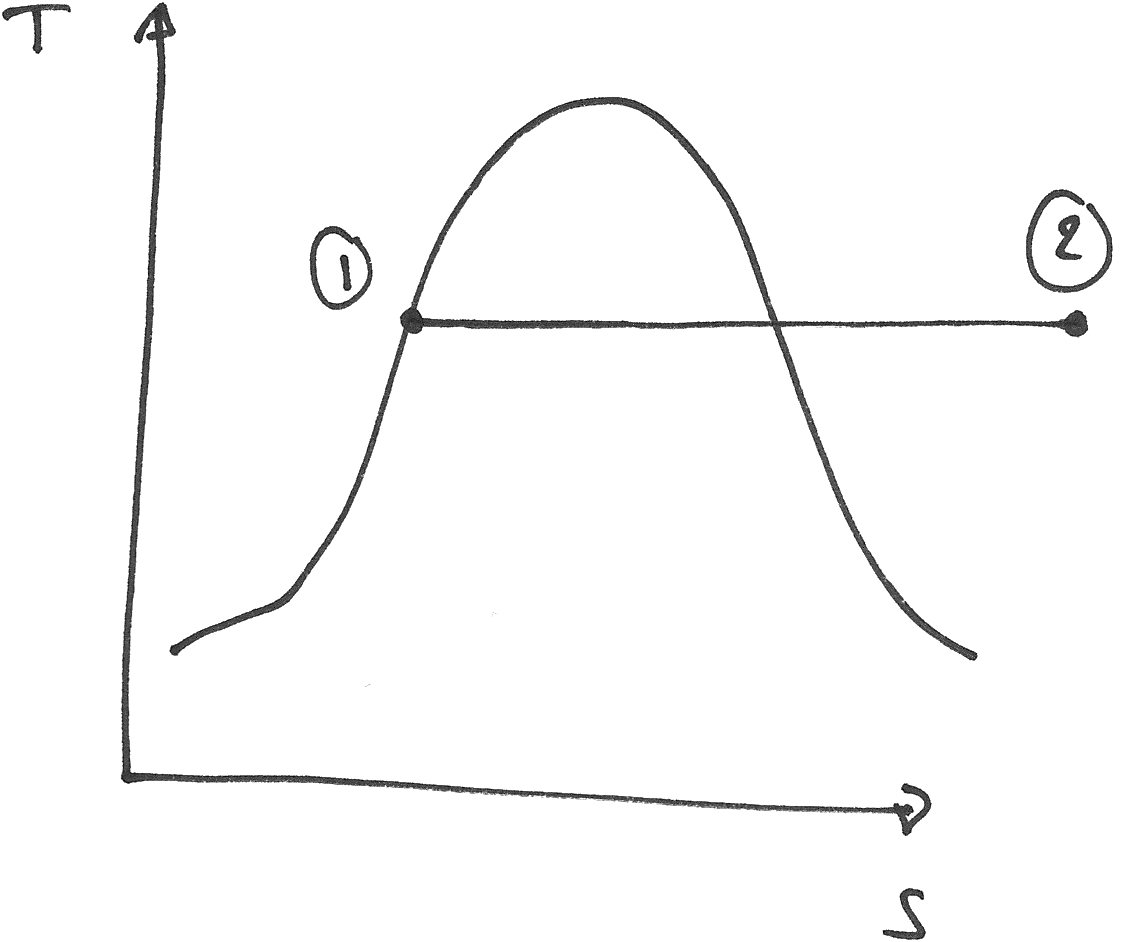
\includegraphics[width=6cm]{images/ts_example_5.png}\end{center}
				Comme l’évolution est réversible nous allons pouvoir calculer $Q_{1\to2}$ en intégrant le terme $T \diff s$ entre $1$ et $2$. \\
				Nous lisons $s_1$ dans l’abaque n°2 : $s_1 = s_{L\SI{300}{\degreeCelsius}} = \SI{3,2552}{\kilo\joule\per\kilogram}$.\\
				À l’arrivée le volume spécifique est $v_2 = \frac{V_2}{m} = \frac{2}{2} = \SI{1}{\metre\cubed\per\kilogram} $ ; pour obtenir $s_2$ il faut interpoler entre deux blocs de l’abaque n°1 (entre \SI{0,2}{\mega\pascal} et~\SI{0,4}{\mega\pascal} à~\SI{300}{\degreeCelsius}). 
				Nous posons $y \equiv \frac{v_2 - v_{\SI{300}{\degreeCelsius}~\&~\SI{0,2}{\mega\pascal}}}{v_{\SI{300}{\degreeCelsius}~\&~\SI{0,4}{\mega\pascal}} - v_{\SI{300}{\degreeCelsius}~\&~\SI{0,2}{\mega\pascal}}} = \frac{1 -\num{1,3162}}{\num{0,65489}-\num{1,3162}} = \num{0,4781} $
				et de façon correspondante, $s_2 = s_{\SI{300}{\degreeCelsius}~\&~\SI{0,2}{\mega\pascal}} + y (s_{\SI{300}{\degreeCelsius}~\&~\SI{0,4}{\mega\pascal}} - s_{\SI{300}{\degreeCelsius}~\&~\SI{0,2}{\mega\pascal}}) = \SI{7,8941} + \num{0,4781}(\num{7,5677}-\SI{7,8941}) = \SI{7,738}{\kilo\joule\per\kelvin\per\kilogram} $.
				
				Nous pouvons donc enfin calculer $q_{1\to2}$ avec l’\cref{eq_q_tds_min} : $Q_{1\to2} = 	\int_1^2 T \diff S = m \ T \Delta s = 2 \times (300+\num{273,15})\times(\num{7,738} - \num{3,2552}) = \SI{+5,139}{\kilo\joule} $.
				
				\begin{remark}Ce calcul un peu laborieux n’est pas nécessairement spectaculaire, mais il faut bien voir que sans l’utilisation de l’entropie, nous n’avions pas de moyen de quantifier $Q_{1\to2}$ sans effectuer d’expérience.\end{remark}\end{answer}
		\end{anexample}
		
		
		\begin{anexample}
			Dans une turbine la vapeur est détendue de façon adiabatique réversible (isentropique). La vapeur entre à~\SI{40}{\bar} et~\SI{500}{\degreeCelsius} ; elle est détendue jusqu’à~\SI{0,5}{\bar}. Quelle est la puissance spécifique fournie ?
			
				\begin{answer}
					Après un coup d’œil aux abaques, l’évolution peut être dessinée de façon approximative sur un diagramme $T-s$ :\\
						\begin{center}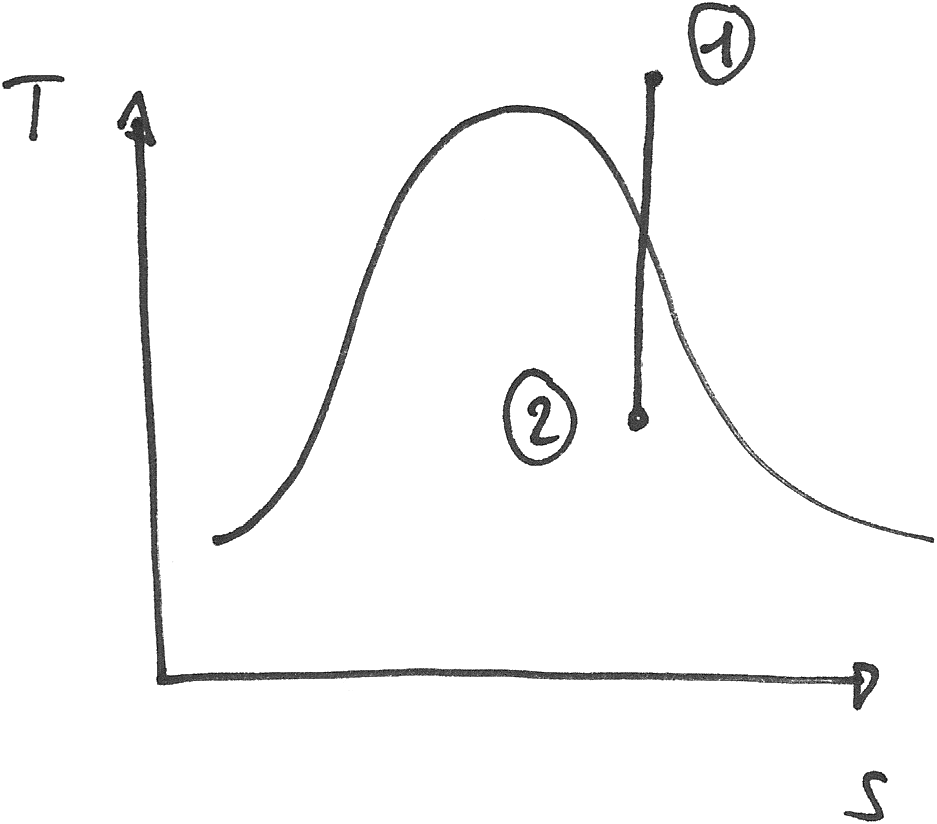
\includegraphics[width=6cm]{images/ts_example_6.png}\end{center}
				Ici $q_{1\to2} = 0$ car la turbine est adiabatique, et nous cherchons $w_{1\to2} = \Delta h$. Il nous faut donc trouver un moyen de quantifier $h_2$.
				
				En $1$ nous lisons dans l’abaque n°1, à~\SI{4}{\mega\pascal} : $h_1 = \SI{3446}{\kilo\joule\per\kilogram}$ et $s_1 = \SI{7,0922}{\kilo\joule\per\kelvin\per\kilogram}$.
				
				En $2$ nous savons que $s_2 = s_1$ car l’évolution est isentropique ; cette information va nous permettre de calculer $h_2$. Dans l’abaque n°2 à~\SI{0,05}{\mega\pascal}, avec l’\cref{eq_titre_entropie} nous obtenons $x_2 = \frac{s_x - s_L}{s_{LV}} = \frac{\num{7,0922}-\num{1,0912}}{\num{6,5018}} = \num{0,923}$. Avec le titre nous pouvons simplement calculer l’enthalpie (\ref{eq_titre_enthalpie}) : $h_2 = h_L + x_2 \ h_{LV} = \num{340,5} + \num{0,923}\times\num{2304,7} = \SI{2467,7}{\kilo\joule\per\per\kilogram}$.
				
				La puissance spécifique de la turbine est donc de $w_{1\to2} = \Delta h = \SI{-978,3}{\kilo\joule\per\kilogram}$.
				
				\begin{remark}Ce procédé est extrêmement utile en ingénierie. L’idée que l’entropie reste constante pendant une évolution adiabatique nous permet (enfin!) de prédire l’état d’un liquide-vapeur à la sortie d’un compresseur ou d’une turbine. Jusqu’à présent, nous pouvions le faire avec un gaz parfait (et les encombrantes relations de type $\frac{T_1}{T_2} = …$), mais pas pour un liquide/vapeur.\end{remark}\end{answer}
		\end{anexample}

\section{Prédire le sens des transformations}

	En quantifiant les variations d’entropie, nous sommes capables de décrire le sens des transformations, c’est-à-dire de prouver par exemple qu’un état B vient \emph{après} un état A. C’est un progrès majeur en physique.

	\subsection{Irréversibilités lors des transferts de chaleur}

		Pour poursuivre convenablement le chapitre, munissons-nous d’une tasse brûlante et insipide de café allemand. Notre intérêt pour la thermodynamique primant sur la boisson, nous collerons notre tasse à une bouteille d’eau fraîche. Ce que nous avons sous les yeux n’est autre qu’une source d’entropie --\ et elle mérite toute notre attention.

		Notre tasse A est à température $T_A$, plus haute que $T_B$, la température de la bouteille d’eau (\cref{fig_expérience_création_entropie}). Les deux corps sont mis en contact et une quantité de chaleur infinitésimale $\diff q$ passe de A vers B.

		\begin{figure}
			\begin{center}
				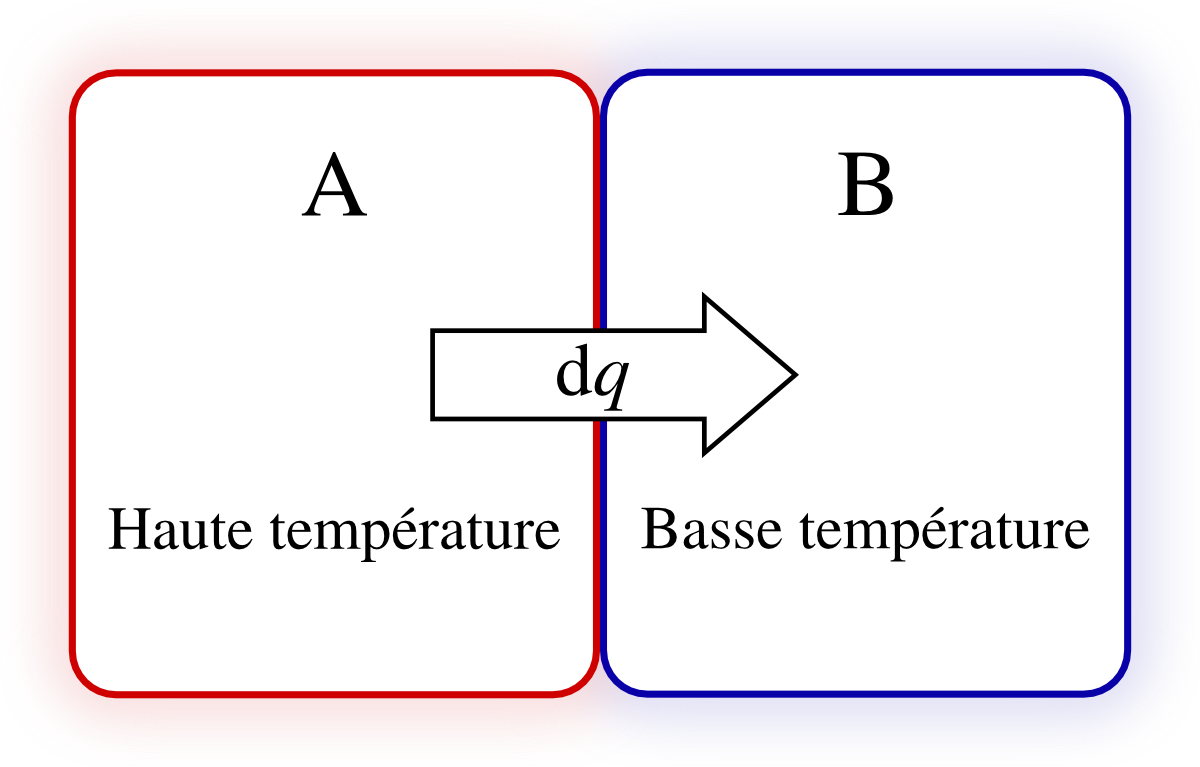
\includegraphics[width=8cm]{images/transfert_chaleur_irreversible.png}
			\end{center}
			\caption{Création d’entropie par transfert de chaleur.
		La transformation est réversible intérieurement pour chacun des deux corps A et B,
		mais irréversible pour le système [A+B].}
			\label{fig_expérience_création_entropie}
		\end{figure}


		Si nous supposons que la température du corps A est homogène,\footnote{Cette «~supposition~» est parfaitement valide dans le cas où $\diff q$ est infiniment petit. Une intégration permet de prendre en compte la variation de température de A au cours de l’échange de chaleur.}
		sa perte de chaleur se fait de façon réversible. Ainsi la variation d’entropie de A est :
		\begin{equation*}
			\diff s_\A = - \frac{\diff q}{T_\A}
		\end{equation*}

		De même, on peut considérer que la température du corps B est homogène : son évolution est réversible intérieurement et la variation de son entropie est :
		\begin{equation*}
			\diff s_\B = + \frac{\diff q}{T_\B }
		\end{equation*}

		Par contre, la température du système entier [A+B] n’est pas du tout homogène : son évolution n’est pas réversible intérieurement. Même si l’ensemble ne reçoit aucune chaleur nette, l’\cref{eq_variation_franche_entropie} ne peut s’appliquer. La variation totale de l’entropie du système [A+B] est :
		\begin{equation}
			\diff s_{[A+B]} = \diff s_\A + \diff s_\B = \frac{\diff q}{T_\B } - \frac{\diff q}{T_\A}
		\end{equation}

		Cette variation est non-nulle ; de l’entropie \textit{a été créée} lors du transfert thermique irréversible. L’irréversibilité n’a lieu ni dans la tasse A, ni dans la bouteille B, mais dans la frontière qui les sépare.

		\begin{figure}
			\begin{center}
				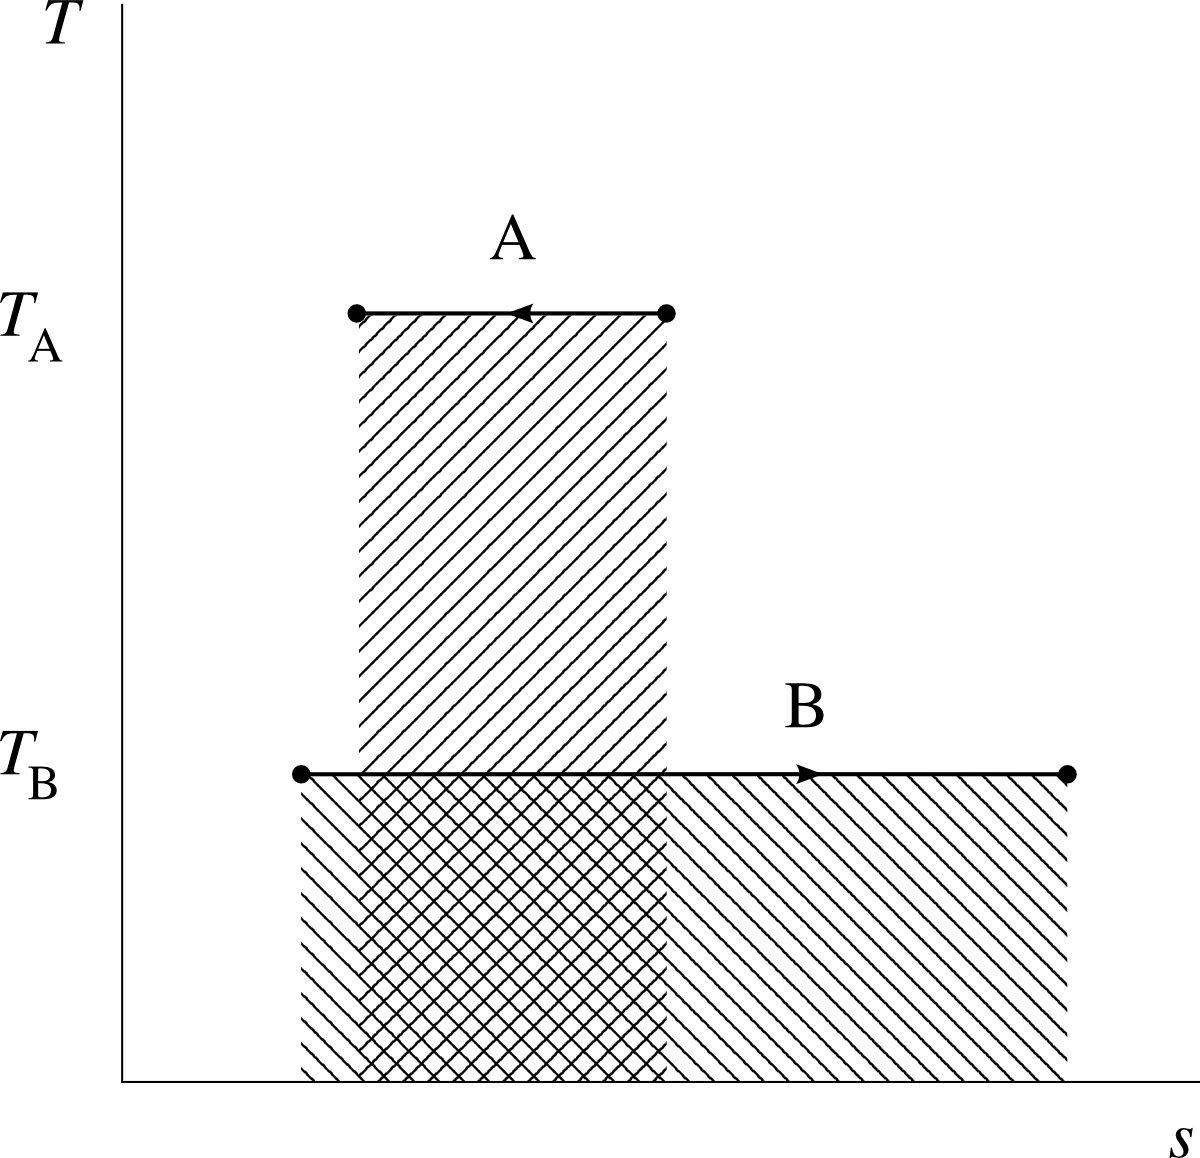
\includegraphics[width=9.5cm]{images/ts_echange_chaleur.png}
			\end{center}
			\caption{Variation d’entropie des corps A et B.
		Les deux aires hachurées sont égales (représentant la quantité de chaleur $\diff q$), mais la somme des deux entropies augmente.}
			\label{fig_expérience_création_entropie_t-s}
		\end{figure}

		Tout gradient de température donne lieu à une irréversibilité, et se traduit par une augmentation de l’entropie totale. On peut se représenter un flux de chaleur entre deux sources de températures différentes par une opportunité perdue de produire un travail\footnote{Et nul ne doute que l’étudiant/e studieux/se, à l’instar de Carnot, trouvera cette situation insupportable…}.
		Ainsi, en plaçant une machine de Carnot entre les corps A et B, aucune irréversibilité n’aurait eu lieu et $\diff s_{[A+B]}$ serait nul. En plaçant une machine thermique de faible rendement, $\diff s_{[A+B]}$ serait faible ; le cas ci-haut où le transfert de chaleur se fait sans machine est le cas limite où aucun travail n’est produit.

		\subsection{Irréversibilités lors des compressions et détentes adiabatiques}

		En pratique, toute détente ou compression se fait en présence d’irréversibilités internes. Comme la durée de l’évolution est finie (contrairement aux évolutions prescrites par Carnot), il y aura nécessairement des déséquilibres de pression au sein du fluide. Ces déséquilibres font apparaître de la turbulence interne, qui provoque la transformation d’énergie cinétique en chaleur, par frottement.

		Ainsi, une compression adiabatique réelle provoque plus d’échauffement du fluide qu’une compression adiabatique réversible (\cref{fig_t-s_détentes_compressions}) : une partie du travail fourni est entièrement convertie en chaleur, au travers des frottements internes.

		Par le même phénomène, une détente adiabatique réelle abaisse moins la température qu’une détente adiabatique réversible. À chaque fois, l’entropie est augmentée bien qu’aucun transfert de chaleur $\diff q$ n’ait eu lieu.
		
		\begin{figure}
			\begin{center}
				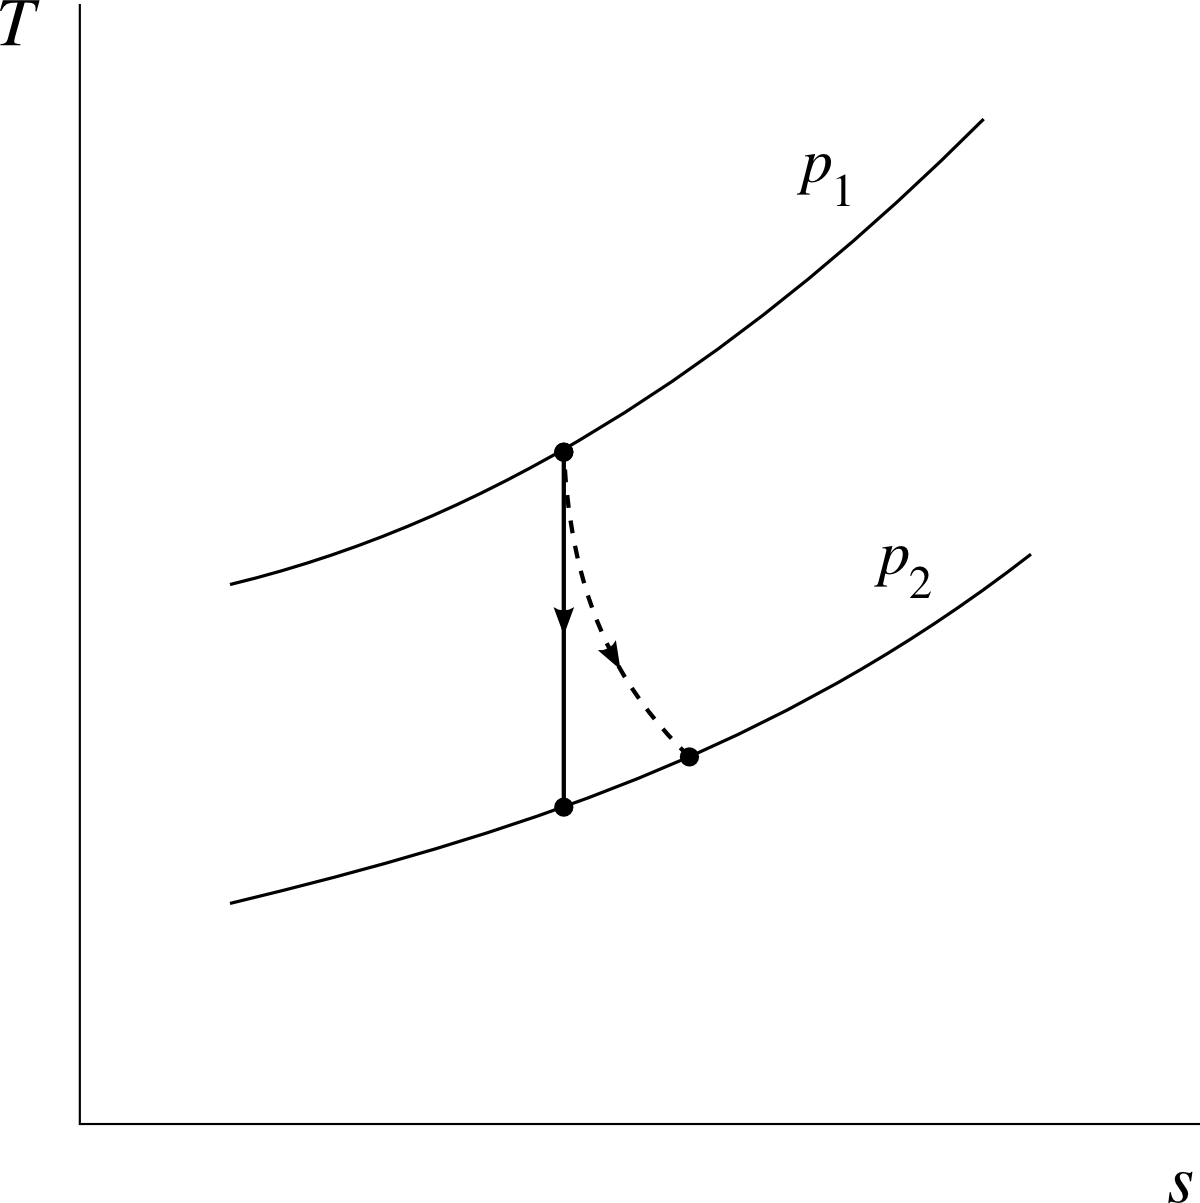
\includegraphics[width=0.45\textwidth]{images/ts_gp_detente.png}
				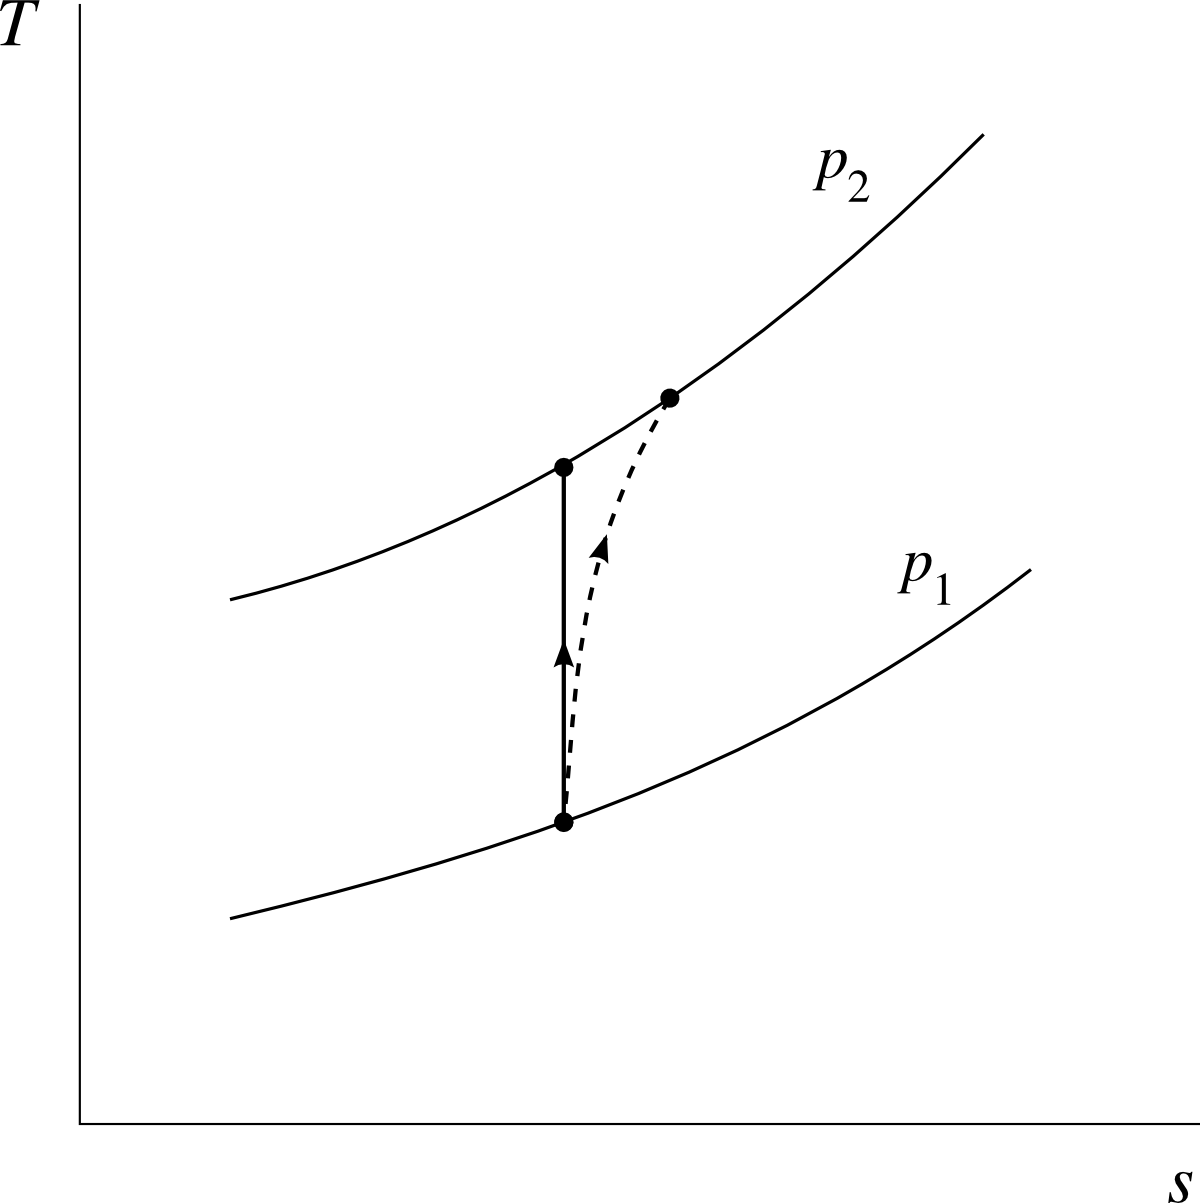
\includegraphics[width=0.45\textwidth]{images/ts_gp_compression.png}
			\end{center}
			\supercaption{Détente et compression adiabatiques théoriques (isentropiques, traits continus)
		et réelles (traits pointillés).\\
		Il faut bien noter que l’accroissement de l’entropie n’est en rien lié à un transfert de chaleur «~$\diff q$~». Le parcours sur le diagramme $T-s$ n’est pas continu et l’aire en dessous ne représente pas un flux de chaleur au travers des frontières du système.}{}
			\label{fig_t-s_détentes_compressions}
		\end{figure}

		

	\subsection{Le second principe et l’entropie}

		Nous avons admis au \courssept que la chaleur ne se déplaçait spontanément que vers une température plus basse --\ un postulat que nous nommons \textit{second principe}. Nous pouvons maintenant formuler cette affirmation avec une expression mathématique.
	
		\begin{description}
			\item[Lors d’un échange de chaleur] d’un corps à température $T_A$ vers un autre à température $T_B$, la variation d’entropie $\Delta s = \frac{-q}{T_\A} + \frac{q}{T_\B }$ est nécessairement nulle ou positive car $T_A$ est nécessairement égale ou supérieure à $T_B$.
			
			\item[Lors d’un échange de travail] toute irréversibilité donne lieu à une température finale plus haute qu’elle n’aurait pu l’être\footnote{La notion de travail irréversible est étudiée au \S\ref{ch_évolutions_irr_sf}.}. L’obtention du même état final avec un chemin réversible demande donc un apport de chaleur, c’est-à-dire un terme $\int \left(\frac{\diff Q}{T}\right)_\text{rév.}$ positif. Une irréversibilité se traduit donc par une augmentation de l’entropie du système.
			
		\end{description}

		Ainsi, nous pouvons traduire le second principe de la façon suivante :
			
		\begin{trucimportant}
			Pour tout système isolé, pour n’importe quelle évolution,
				\begin{equation}
					\Delta s \geqslant 0
					\label{eq_augmentation_entropie}
				\end{equation}
		\end{trucimportant}

		On peut toujours réduire l’entropie d’un système pour la ramener à sa valeur initiale (il suffit pour cela de le ramener à son état initial), mais cela se fera nécessairement au prix d’une augmentation \emph{au moins aussi grande} de celle d’un autre système.


	\subsection{Prédire le sens des transformations}
	
		Si l’on veut montrer qu’un système ne peut aller que d’un état A à un état B, c’est-à-dire que l’évolution est irréversible, il nous faut procéder de la façon suivante :
	
		\begin{enumerate}
			\item Il faut trouver un chemin réversible $\A \to \B$, c’est-à-dire un procédé pour aller de A à B en gardant toujours la pression et la température homogènes même si elles varient ;
			\item Le long de ce chemin réversible, nous calculons $\Delta s$ (c’est-à-dire que nous effectuons l’intégrale $\int \frac{\diff q}{T} $ pour ce chemin).
			\item Nous comparons avec l’intégrale $\int \frac{\diff q}{T} $ le long du chemin \emph{réel}, qui elle ne correspond pas à la variation d’entropie.
		\end{enumerate}

		Il y a trois possibilités :
			\begin{itemize}
				\item Si les deux intégrales sont égales, alors la transformation réelle est \vocab{réversible} : elle peut avoir lieu dans les deux sens.
				\item Si $\int \left(\frac{\diff q}{T}\right)_\text{chemin réel} < \int \left(\frac{\diff q}{T}\right)_\text{rév.}$, alors la transformation réelle est \vocab{irréversible}. Elle ne peut avoir lieu que dans ce sens.
				\item Si $\int \left(\frac{\diff q}{T}\right)_\text{chemin réel} > \int \left(\frac{\diff q}{T}\right)_\text{rév.}$, alors la transformation «~réelle~» décrite est \vocab{impossible}. Elle ne peut avoir lieu que dans le sens inverse (B $\to$ A). 
			\end{itemize}
			
		Même si dans ce chapitre nous ne savons calculer ces intégrales que pour des transformations et des fluides simples, cette démarche reste valide pour toute évolution (une pierre jetée dans un étang, une assiette qui se casse en tombant). C’est une étape majeure en physique, que nous n’avons franchie qu’en 1865 (grâce à \wf{Rudolf Clausius}).

		\begin{anexample}
			Une masse d’air suit une évolution sans apport de chaleur. Il y a deux états :
				\begin{itemize}
					\item Un état $X$ à~\SI{5}{\bar} et~\SI{100}{\degreeCelsius} ;
					\item Un état $Y$ à~\SI{1}{\bar} et~\SI{5}{\degreeCelsius}.
				\end{itemize}
			Quel est le seul sens ($X \to Y$ ou $Y \to X$) dans lequel l’évolution peut avoir lieu ?
						
				\begin{answer}
					Proposons le sens $X \to Y$ et vérifions s’il est physiquement possible.
					
					La variation d’entropie est égale à l’intégrale $\int_X^Y \left(\frac{\diff q}{T}\right)_\text{rév.}$. Avec l’\cref{eq_delta_s_gp_p}, $\Delta s = c_p \ln \frac{T_Y}{T_X} - R \ln \frac{p_Y}{p_X} = \num{1005} \ln \frac{5+273,15}{100+273,15} - \num{286} \ln\frac{1}{5}=  \SI{+166,6}{\joule\per\kelvin\per\kilogram}$.

					De l’autre côté, l’intégrale $\int_X^Y \left(\frac{\diff q}{T}\right)_\text{chemin réel}$ est égale à zéro car en réalité il n’y a pas eu de transfert de chaleur ($\diff q = 0$).
					
					Nous avons donc $\Delta s > \int_X^Y \left(\frac{\diff q}{T}\right)_\text{chemin réel}$ et l’évolution est irréversible. Si nous voulions revenir en arrière, de $Y$ à $X$, nous serions obligés de retirer de la chaleur.		
					L’évolution peut être dessinée de façon approximative sur un diagramme $T-s$ :\\
						\begin{center}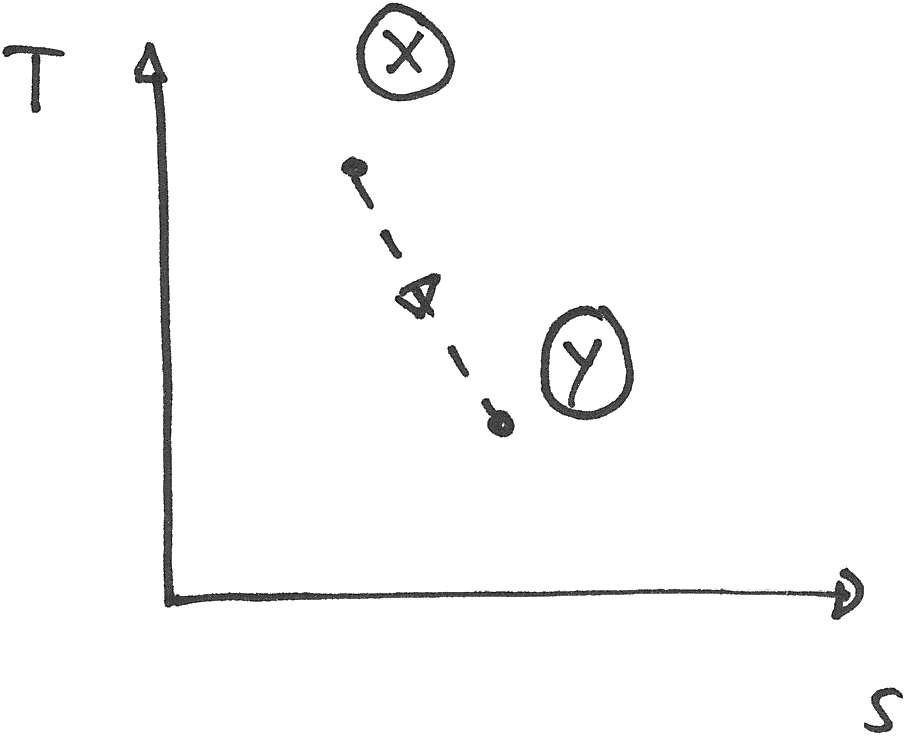
\includegraphics[width=6cm]{images/ts_example_7.png}\end{center}
				\end{answer}
		\end{anexample}

		

		\begin{anexample}
			De l’eau suit une évolution pendant laquelle on lui apporte \SI{1}{\mega\joule\per\kilogram} de chaleur (sa température étant alors figée à~\SI{130}{\degreeCelsius}). Il y a deux états, un au début et l’autre à la fin :
				\begin{itemize}
					\item Un état $X$ à l’état de liquide saturé à~\SI{130}{\degreeCelsius} ;
					\item Un état $Y$ à l’état de vapeur saturée à~\SI{170}{\degreeCelsius}.
				\end{itemize}
			Quel est le seul sens ($X \to Y$ ou $Y \to X$) dans lequel l’évolution peut avoir lieu ?
						
				\begin{answer}
					Proposons le sens $X \to Y$ et vérifions s’il est physiquement possible.
					
					Nous lisons les valeurs de l’entropie dans l’abaque n°2 : $s_X = s_{L \SI{130}{\degreeCelsius}} = \SI{1,6346}{\kilo\joule\per\kelvin\per\kilogram}$ et $s_Y = s_{V \SI{170}{\degreeCelsius}} = \SI{6,665}{\kilo\joule\per\kelvin\per\kilogram}$. \\
					Ainsi, $\Delta s = \int_X^Y \left(\frac{\diff q}{T}\right)_\text{rév.} = \SI{+5,03}{\kilo\joule\per\kelvin\per\kilogram}$.
					
					De l’autre côté, nous pouvons calculer l’intégrale $\int_X^Y \left(\frac{\diff q}{T}\right)_\text{chemin réel}$ car nous savons que la chaleur a été apportée lorsque la température était fixée à~\SI{130}{\degreeCelsius}. Ainsi $\int_X^Y \left(\frac{\diff q}{T}\right)_\text{chemin réel} = \frac{1}{T} \int_X^Y \left(\diff q\right)_\text{chemin réel} = \frac{q_{X\to Y}}{T} = \frac{\num{1e6}}{170+273,15} = \SI{+2,26}{\kilo\joule\per\kelvin\per\kilogram}$.
					
					L’évolution peut être dessinée de façon approximative sur un diagramme $T-s$ :\\
						\begin{center}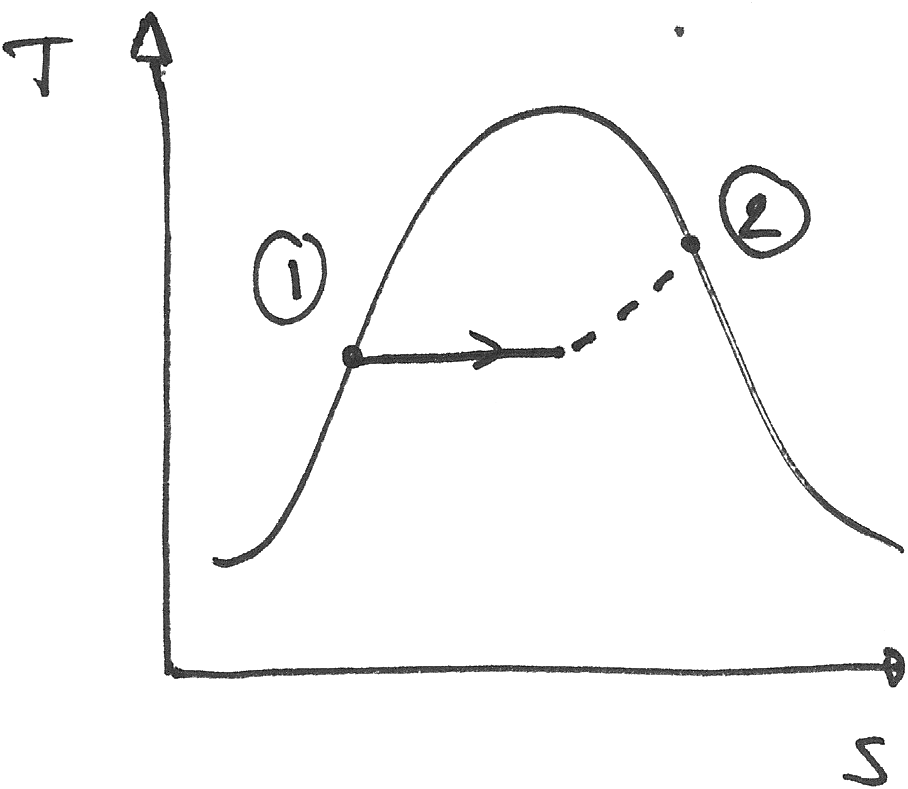
\includegraphics[width=6cm]{images/ts_example_8.png}\end{center}
					
					Ici, nous avons $\Delta s > \int_X^Y \left(\frac{\diff q}{T}\right)_\text{chemin réel}$ et l’évolution est irréversible. Si nous voulions revenir en arrière, de $Y$ à $X$, nous serions obligés de refroidir le gaz en lui retirant \emph{nécessairement} une quantité plus grande que \SI{1}{\mega\joule\per\kilogram}.
				
				\end{answer}
		\end{anexample}

\section{L’entropie et l’univers}

	\subsection{À quoi sert l’entropie ?}

		C’est une question légitime mais qui n’a pas beaucoup plus de sens que la question «~à quoi sert l’énergie ?~». Tout comme l’énergie, l’entropie est une notion difficile à appréhender et conceptualiser, et dont l’utilité vient lorsqu’on quantifie ses variations.
		
		Pour l’ingénieur/e, nous retiendrons que la quantification des variations d’entropie permet deux choses :
		\begin{enumerate}
			\item L’entropie est «~ce qui ne varie pas lorsque l’on comprime et détend les fluides de façon idéale~». Elle nous permet de quantifier les propriétés que devrait avoir un liquide/vapeur à la sortie d’un compresseur ou d’une turbine.
			\item L’entropie est «~ce qui ne peut qu’augmenter dans un système isolé lorsqu’il se transforme~». Elle nous permet de prédire dans quel \emph{sens} une transformation peut ou ne peut pas avoir lieu.
		\end{enumerate}

	\subsection{Contexte}
	
		L’entropie a été introduite par \wf{Rudolf Clausius} en 1865 pour exprimer de façon mathématique ce que nous connaissons aujourd’hui sous le nom de second principe. Clausius résume l’ensemble des connaissances contemporaines dans une publication magistrale --\ \textit{Über verschiedene für die Anwendung bequeme Formen der Hauptgleichungen der mechanischen Wärmetheorie}\ -- dans laquelle il conclut une décennie de travail autour de la grandeur $\frac{Q}{T}$.
		
		Sa référence étymologique au grec et les explications à propos du «~contenu de changement\footnote{\textit{Verwandlungsinhalt}, de ses propres mots.}~» qu’il utilise pour créer le terme \vocab{entropie} ne l’aident pas beaucoup. La notion d’entropie, vite détestée (à tort !) de tous les étudiants, est pourtant universellement acceptée. Pour l’ingénieur/e, la science de «~savoir ce qu’est la chaleur~», fraîchement nommée \vocab{thermodynamique}, vient juste d’être conclue.
		
	\subsection{Pour aller plus loin}
	
		Il est difficile de conclure un chapitre sur l’entropie avant d’avoir mentionné la quantification que propose \wf{Ludwig Boltzmann} en 1875 :
			
			\begin{equation}
				S = k \ln \lambda
			\end{equation}
			
			\begin{equationterms}
				\item où \tab $\lambda$ \tab est le nombre de configurations possibles du système qui correspondent à son état, 
				\item et \tab $k$ \tab est une constante.
			\end{equationterms}
		
		Ainsi pour Boltzmann l’entropie est une mesure de la probabilité du système d’être dans cet état. Plus la configuration est probable (homogénéité de la pression et de la température), plus l’entropie est grande.
		
		Il reste des difficultés inhérentes liées à la quantification de~$k$ et surtout de~$\lambda$ ; mais le pont est établi avec le monde des probabilités et statistiques. On parle alors de \vocab{thermodynamique microscopique} ou \vocab{statistique}, domaines de la physique qui ne concernent plus directement l’ingénieur/e.
		
	\subsection{L’entropie et l’univers}
	
		Dans la mesure où l’on pense à l’univers comme à un ensemble fini, c’est-à-dire comme à un système isolé contenant une quantité fixe d’énergie, on ne peut que se demander si l’on ne peut lui appliquer l’\cref{eq_augmentation_entropie}. Clausius est sans équivoque : il termine son article de 1865 par l’affirmation :
			
			\begin{quote}
				Si l’on imagine que l’on ait calculé d’une manière conséquente pour l’univers entier […] la quantité que j’ai nommée \textit{entropie} pour un corps particulier, ainsi que la quantité désignée sous le nom d’\textit{énergie} et dont le sens est plus facile à saisir, on pourra exprimer très simplement, sous la forme suivante, les lois fondamentales de l’univers qui correspondent aux deux principes essentiels de la théorie mécanique de la chaleur :
					\begin{enumerate}
						\item L’énergie de l’univers est constante.
						\item L’entropie de l’univers tend vers un maximum.
					\end{enumerate}
			\end{quote}
		
		On voit qu’en partant du fonctionnement des moteurs, on est arrivé à des notions extrêmement puissantes. L’univers se comporte-t-il comme la vapeur d’eau de nos centrales ? Pour explorer cette question de façon ludique, l’étudiant/e pourra lire \textit{\href{http ://www.multivax.com/last_question.html}{The Last Question}} d’Isaac Asimov ou \textit{\href{http ://www.eyrolles.com/Sciences/Livre/l-entropie-et-tout-ca-9782842250447}{L’entropie et tout ça}} de Philippe Depondt. Pour une réponse plus formelle, il faudra se reporter à un bon manuel de physique.
